\section{Discussion}
\label{sec:discussion}

In this section, we discuss our selected examples, then give a walk through of working with a complex prompt, and finally provide a break-down (with examples) of limitations of \bdraw.

\subsection{Selected Examples}
\label{sec:selected_discussion}

In Figures \ref{figs:teaser} and \ref{figs:cherries} (along with the additional examples in Figures \ref{figs:appendix_cherry1}, \ref{figs:appendix_cherry2} and \ref{figs:appendix_cherry4} in the Appendix), we hope to concretely convey some of the strengths of \bdraw, including its ability to handle complex prompts, multiple visual styles, words-on-text, world knowledge, and more. The top row of Figure \ref{figs:teaser} shows the model accommodating a very long and complex description of van Gogh's painting The Starry Night---the outputs all come from the same batch and show considerably visual diversity. The other rows show that the model can co-locate famous landmarks in a common scene and adapt styles.

The top row of Figure \ref{figs:cherries} shows single images for tricky or complex prompts: (A) is short but includes writing of an intentionally misspelled word ``toaday'' (toad-ay) and an image-within-image specification that is successfully executed; (B) has a complex prompt that requires knowledge of both Anubis and the Los Angeles skyline; and (C) has extensive visual complexity covering multiple entities and their details and (literal) writing on the wall, with photo-realism. (D) shows simple but effective concept combination. (E) provides four outputs from the same batch, showing both diversity and quality of multiple outputs for a complex prompt. (F) demonstrates text rendering of a reasonably long expression along with other complex details, including following the contours of driftwood, fading of the writing and its reflection in the water, and integration of words into stained glass.\footnote{The prompts in Figure \ref{figs:cherries}, panel F are: \textit{The saying "BE EXCELLENT TO EACH OTHER" X}, where X is: \begin{itemize}[itemsep=0.5pt]
    \item \textit{written on a red brick wall with a graffiti image of a green alien wearing a tuxedo. A yellow fire hydrant is on a sidewalk in the foreground.}
    \item \textit{written with carved letters on driftwood.}
    \item \textit{written in faded paint on the hull of an old wooden boat and reflected in the water. Wide-angle lens.}
    \item \textit{written in a stained glass window.} \end{itemize}} (G) shows that the model can reproduce world knowledge related to precise visual details for multiple variants of three vehicles that have existed and changed over many decades, while also incorporating additional scene details and color specifications and producing photo-realistic outputs. (H) shows a detailed description in the style of various artists and art movements. (I) shows the adaptation of animals and sports to the style of Egyptian hieroglyphics and additionally placed on Athenian vases (which featured a different art style), including conforming the painting to the contours of the vases.

\subsection{Growing a Cherry Tree}\label{secs:growing_cherry_tree}
\begin{figure}
\centering
\begin{adjustwidth}{-0.8in}{-0.9in}
\centering
    \vspace{-1cm}
    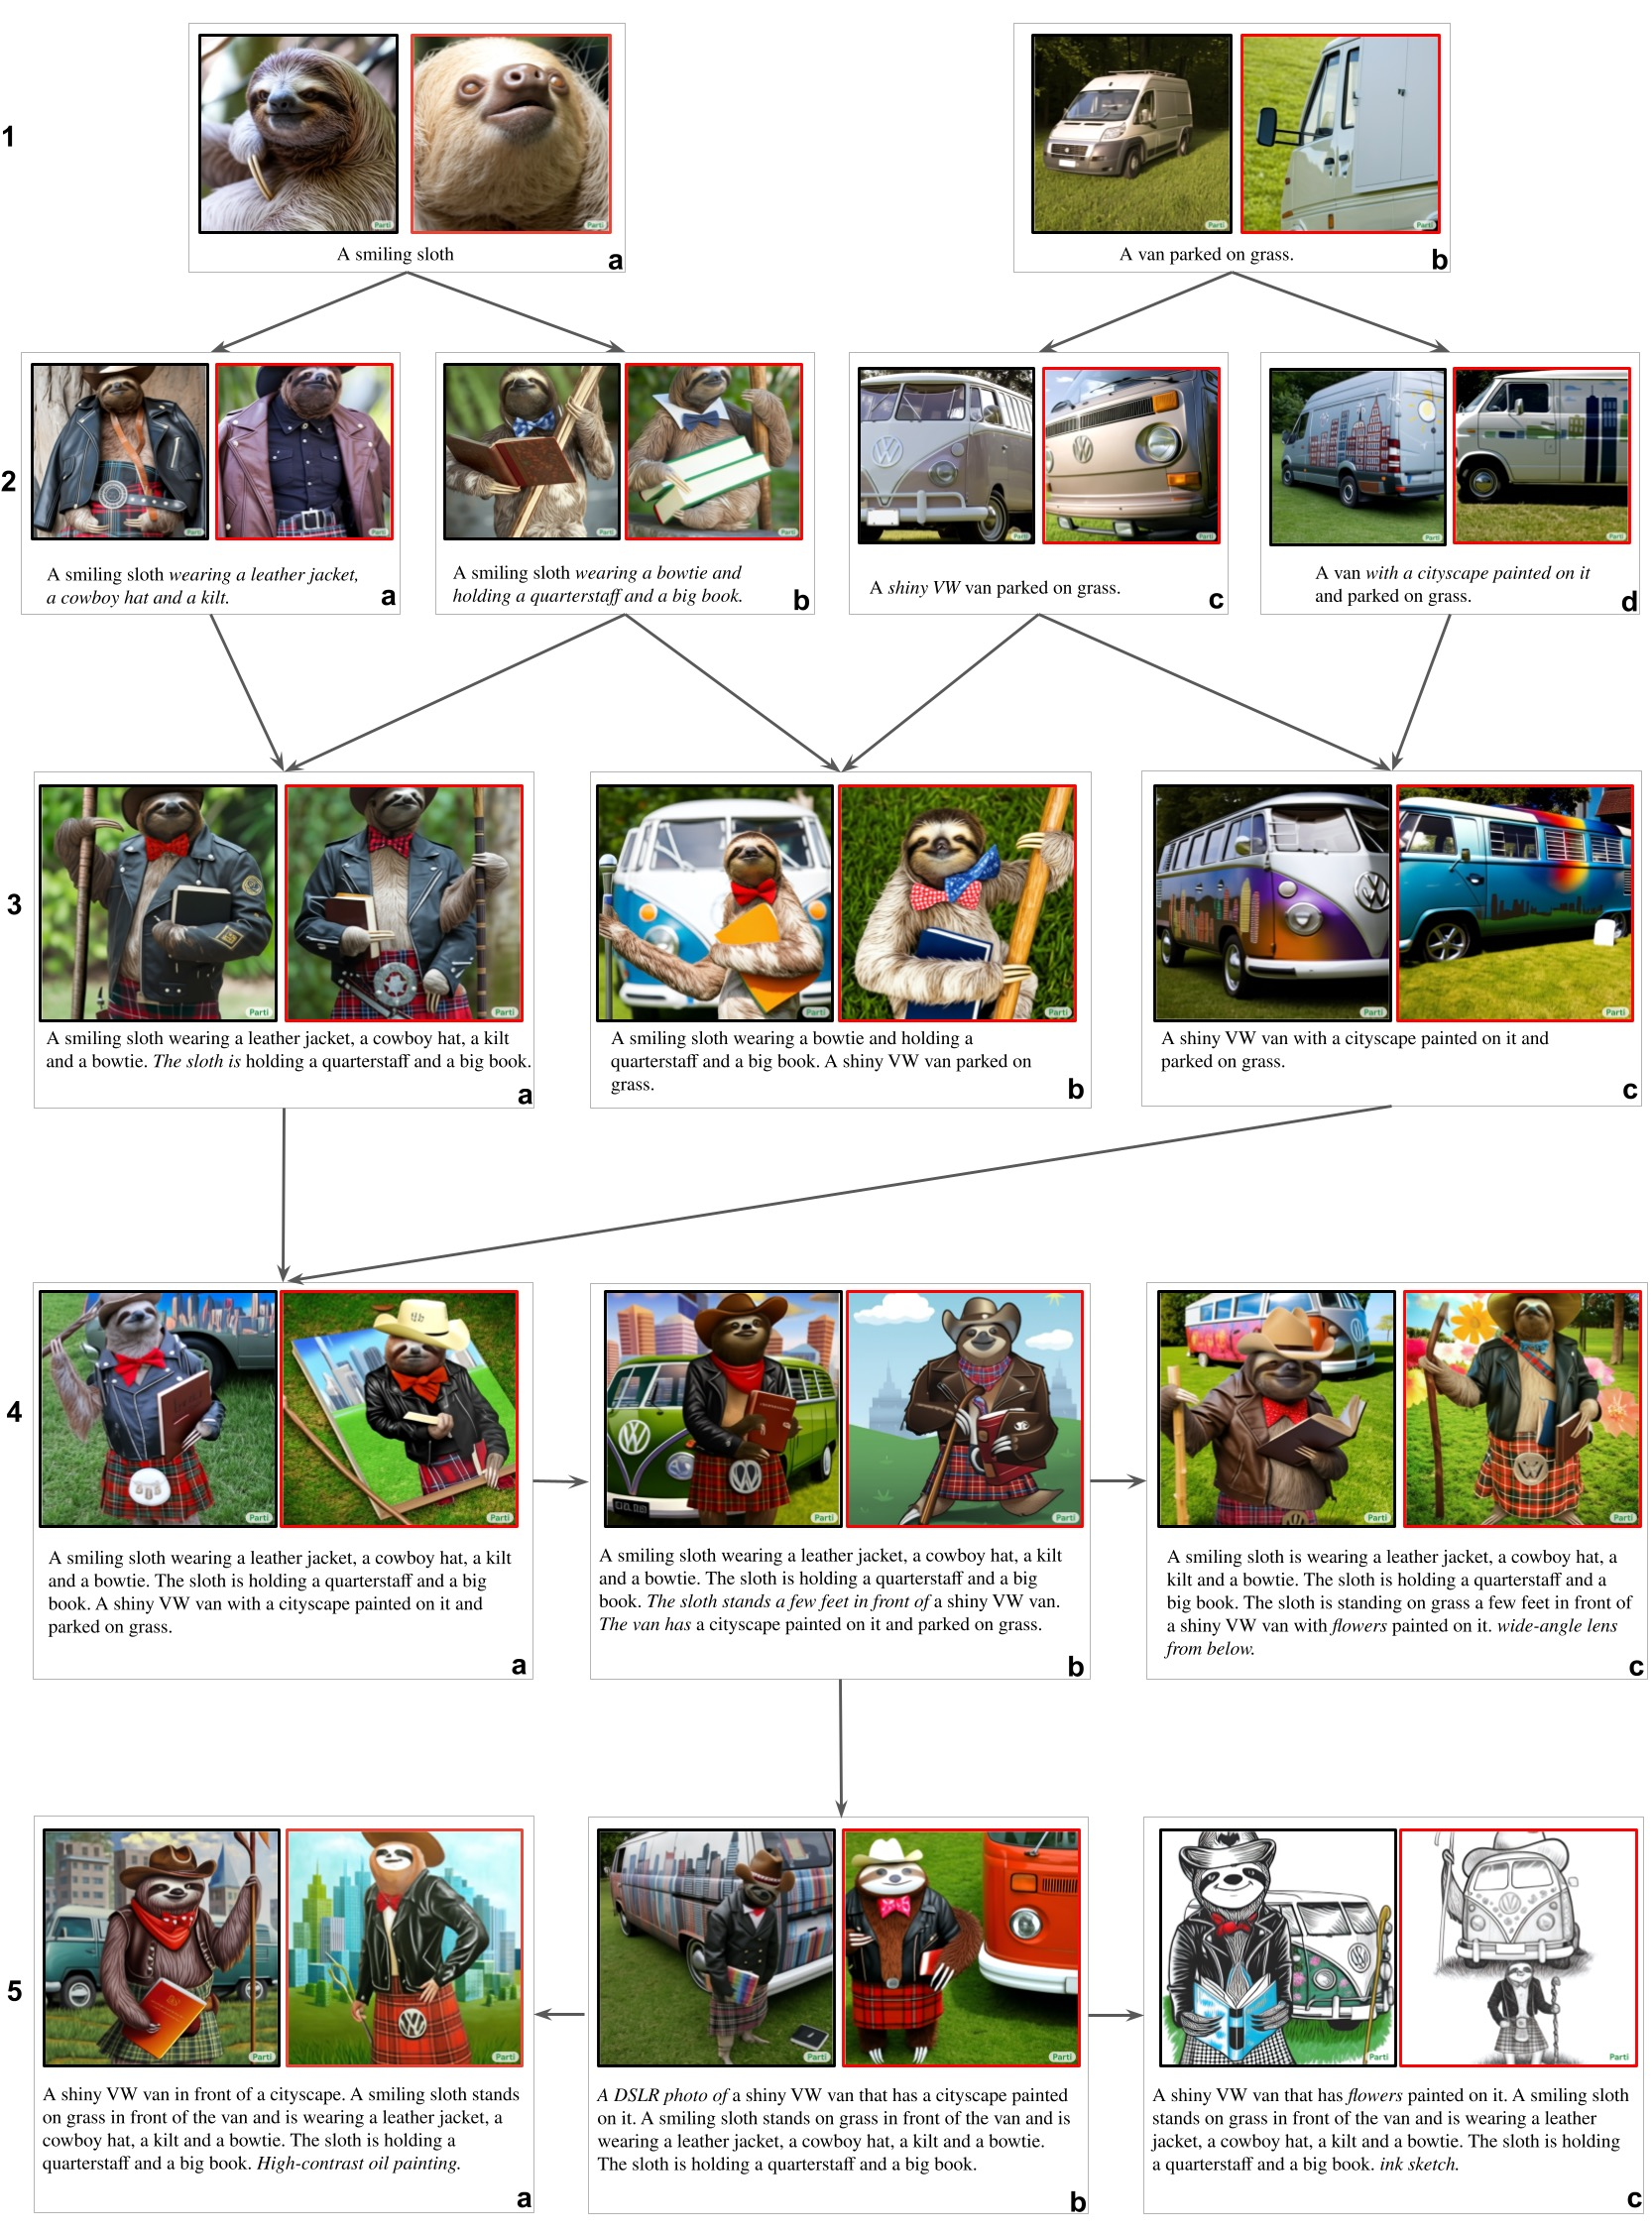
\includegraphics[scale=0.25]{figures/growing_cherry_tree.jpg}
\end{adjustwidth}
\caption{A depiction of several steps in the process of adding details or rephrasing to build a complex prompt that the model responds to well. For each prompt, we show the best output of the top eight ranked images (on the left) and the worst (on the right), using the 20B \bdraw model. Note that for rows 1-4, the additional text ``\textit{dslr photograph. daytime lighting.}'' is appended to the given prompt. See Section~\ref{secs:growing_cherry_tree} for discussion.}
\label{figs:cherry_tree}
\end{figure}

Like other recent work on text-to-image generation, this paper includes novel images and the complex prompts given to the model to produce them, as discussed in the previous subsection. Naturally, the most challenging and impressive examples are \textit{selected} (that is, \textit{cherry picked}), as noted in the captions. As such, they do not typically represent, for example, a single shot interaction in which the model directly produces such an image as its most highly ranked output. As noted in section \ref{secs:broader}, we are unable to release our model directly to the public, so in this section we hope to provide a brief window into the process of increasing descriptive and visual complexity with \bdraw, including how, along the way, things go right or do not just work immediately.

A key concept we would like to introduce in this endeavor is that of \textit{growing the cherry tree} --- a concept that we believe will be useful in this space going forward. To put a fine point on it, many of the prompts and resulting images that are seen in Figure \ref{figs:cherries} and others in the Appendix (noted as ``selected'') are not only cherry picked: they are the result of exploring and probing the model's capabilities -- the product of an interactive process in which a prompter tests a prompt idea, evaluates the outputs holistically, modifies the prompt, and repeats the process. Sometimes, all the outputs are great, and the prompter wants to push the model further. Other times, none of the outputs are ideal, so strategies to change or rephrase the prompt are employed. In this way, one develops a prompt in increments while interacting with the model, in order to produce a cherry tree that offers up some great outputs that can ultimately be plucked. While many--perhaps most--of the prompts an average user would come up with would be quite a bit simpler, this is how we find the breaking points and identify the next opportunities and challenges to focus on. We also expect that designers, artists and other creatives would similarly want to push on these limits; anecdotally, this is how some artists have described working with current text-to-image models that are available to the public.

As a concrete example, consider the process of developing a complex prompt as depicted in Figure \ref{figs:cherry_tree}. This shows a branching and merging process of creating prompt variations, along with two outputs for each prompt. In each box with a prompt, the best of the top eight 20B \bdraw outputs (as ranked from all outputs) is given on the left and the worst of the top eight is given on the right. 

\begin{itemize}
    \item We start with two core entities, the sloth and the van, in Row 1. 
    \item Row 2 adds specific details for each; overall, the model accommodates this well, but notice that box 2(b) has a sloth with two books and an odd bow tie as its worst outcome of eight.
    \item Row 3 shows the first major problems: Box 3(a) has two left arms on the sloth and Box 3(b) has a sloth but is completely missing the van mentioned in the prompt.
    \item Row 4 shows where things start to get particularly tricky: 4(a) is the full combination of the sloth and van with all details, though only by simple concatenation of the respective prompts. The best (left) output manages to get things technically correct, but the van is out of the picture; however, the worst (right) output is a confused mess. 4(b) attempts to improve matters by relating the sloth and van via positioning (\textit{The sloth stands a few feet in front of a shiny VW van}), but this ends up producing cartoonish outputs, and even the best output puts the cityscape in the background rather than on the van. 4(c) shows one fix, which is to switch to flowers on the van; with this, the model can produce a strong, photorealistic output that corresponds well with the prompt.
    \item A second fix is given in 5(b), where the van and photo are promoted to the front of the prompt (rephrasing); alas, the sloth is missing its quarterstaff in the best output, and the worst output is cartoonish and lacking in key details. 5(a) shows that some problems of perspective and representation are resolved by going to a non-photo format (but the city is not on the van, yet again). 5(c) shows that a format change (to \textit{ink sketch}) and swapping flowers for the cityscape again rescue the composition for the best output; however, the worst output is again a confused mess with a van that has a cowboy hat and a sloth arm holding a quarterstaff. 
\end{itemize}

We hope this diagram and its description give a sense of how a model like this responds as one adds detail and rephrases prompts. In a sense, this is a form of \textit{model whispering} as one stretches such models to their limits. That said, it is often remarkable how much descriptive complexity and diversity the model can readily accommodate. In the next section, we point to specific areas in which the \bdraw model still systematically runs into difficulty and are thus key areas for improvement.

\subsection{Limitations}
\label{secs:limitations}

There are a number of situations that \bdraw currently handles poorly or inconsistently, or which lead to interesting patterns in outputs -- even producing some bloopers (which can at times be delightful). The likelihood of all of these errors increases with prompt complexity. Figure \ref{figs:limitations} provides example prompts and images, along with mention of specific failure modes they exemplify. Note that the examples are selected \textit{non-cherries} that are often low in the ranked outputs, and that in many cases (though not all) the model produces a highly ranked and high-quality output for the prompt. \footnote{Some prompts could not fit in the figure. They are: \begin{itemize}[itemsep=0.5pt]
    \item[\textbf{H(a,b)}] \textit{A robot painted as graffiti on a brick wall. The words "Fly an airplane" are written on the wall. A sidewalk is in front of the wall, and grass is growing out of cracks in the concrete.}
    \item[\textbf{I(a,b)}] \textit{Horses pulling a carriage on the moon's surface, with the Statue of Liberty and Great Pyramid in the background. The Planet Earth can be seen in the sky. DSLR photo.}
    \item[\textbf{I(c)}] \textit{A shiny robot wearing a race car suit and black visor stands proudly in front of an F1 race car. The sun is setting on a cityscape in the background. comic book illustration.}
    \item[\textbf{I(d)}] \textit{the saying "BE EXCELLENT TO EACH OTHER" on a rough wall with a graffiti image of a green alien wearing a tuxedo.} \end{itemize}} We list the failure modes and discuss them here. Unless otherwise specified, all references are to Figure \ref{figs:limitations}, and are given in terms of panel (capital letter) and image (a-d).
 
\begin{figure}
\begin{adjustwidth}{-0.8in}{-0.5in}  
    \centering                     
    \footnotesize
\setlength\tabcolsep{2pt}
\vspace{-0.5in}
\begin{tabular}{cccccccccccccccccccc}

\multicolumn{3}{c}{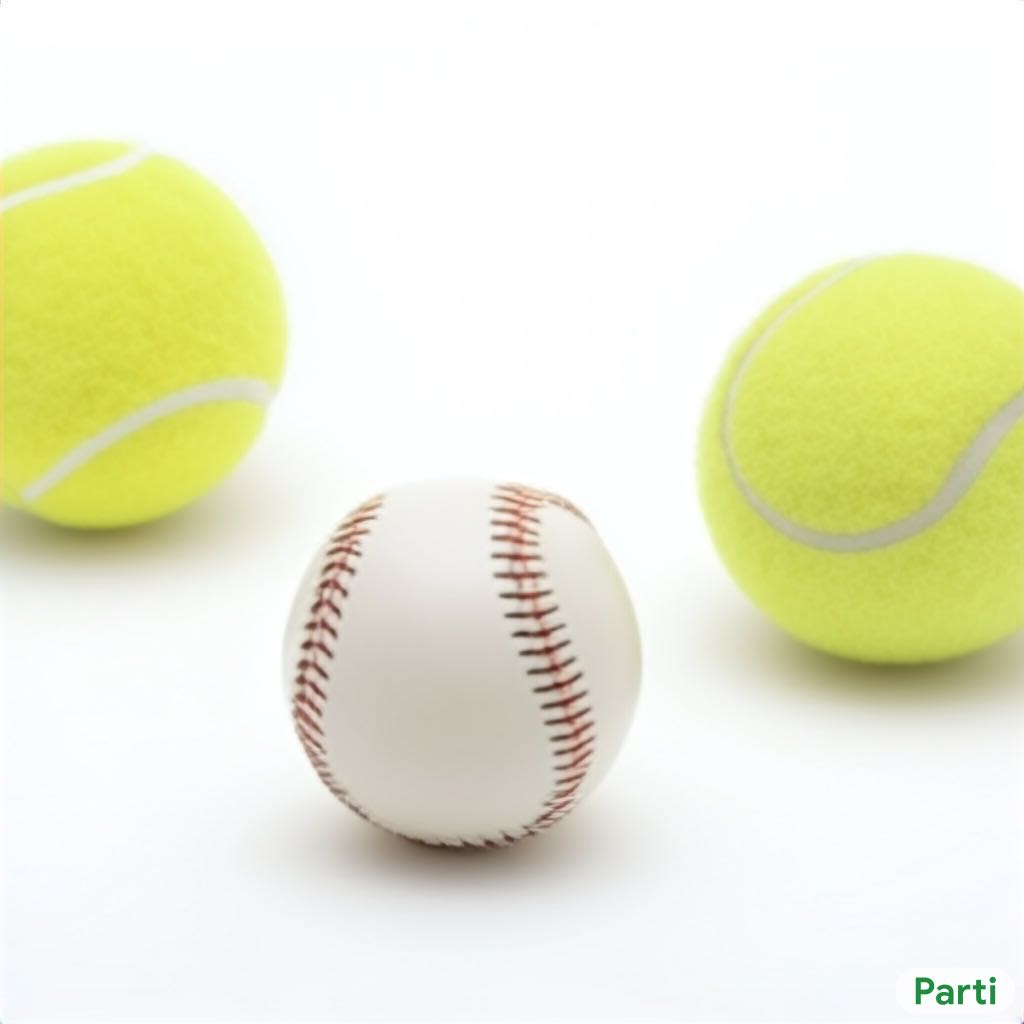
\includegraphics[width=\twobytwocolwidth\textwidth]{figures/limitations/2tennis1baseball.jpg}} &
\multicolumn{3}{c}{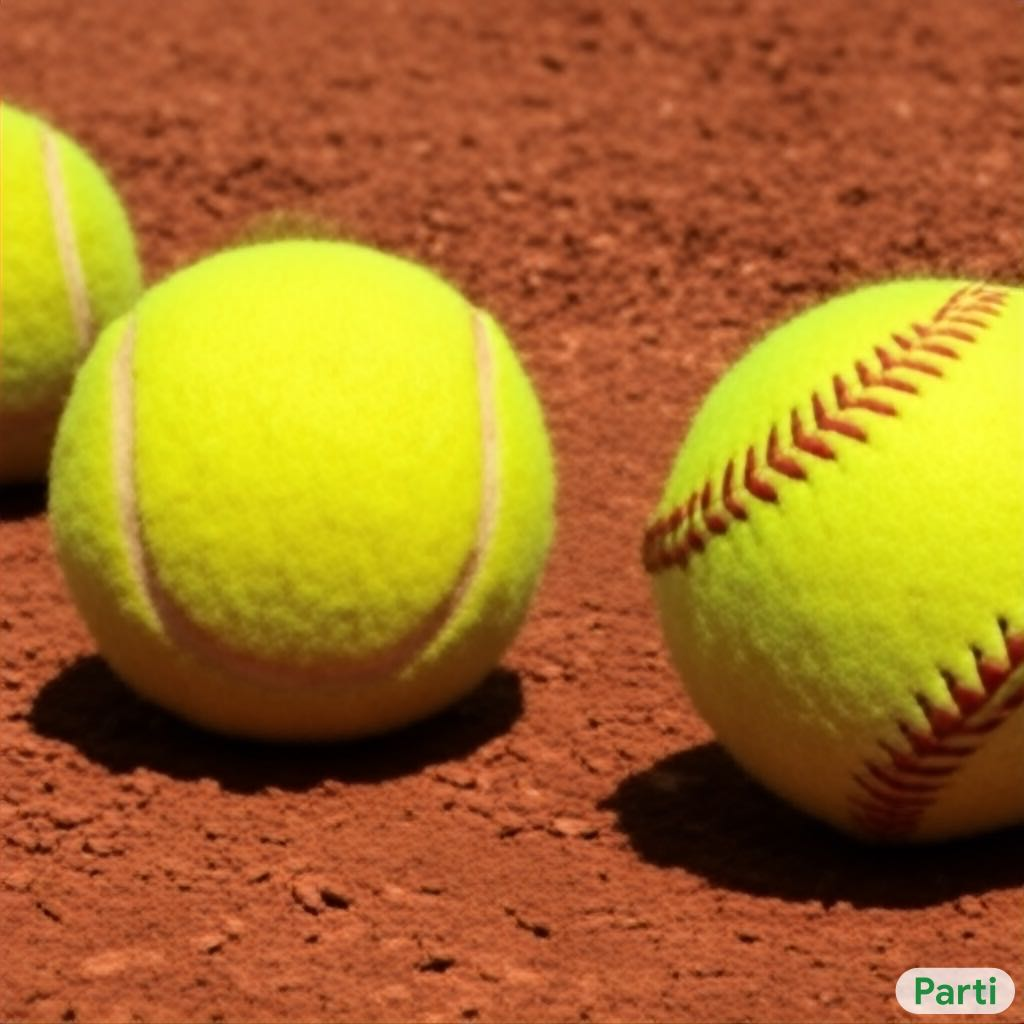
\includegraphics[width=\twobytwocolwidth\textwidth]{figures/limitations/2tennis1mergedball.jpg}} &&
\multicolumn{3}{c}{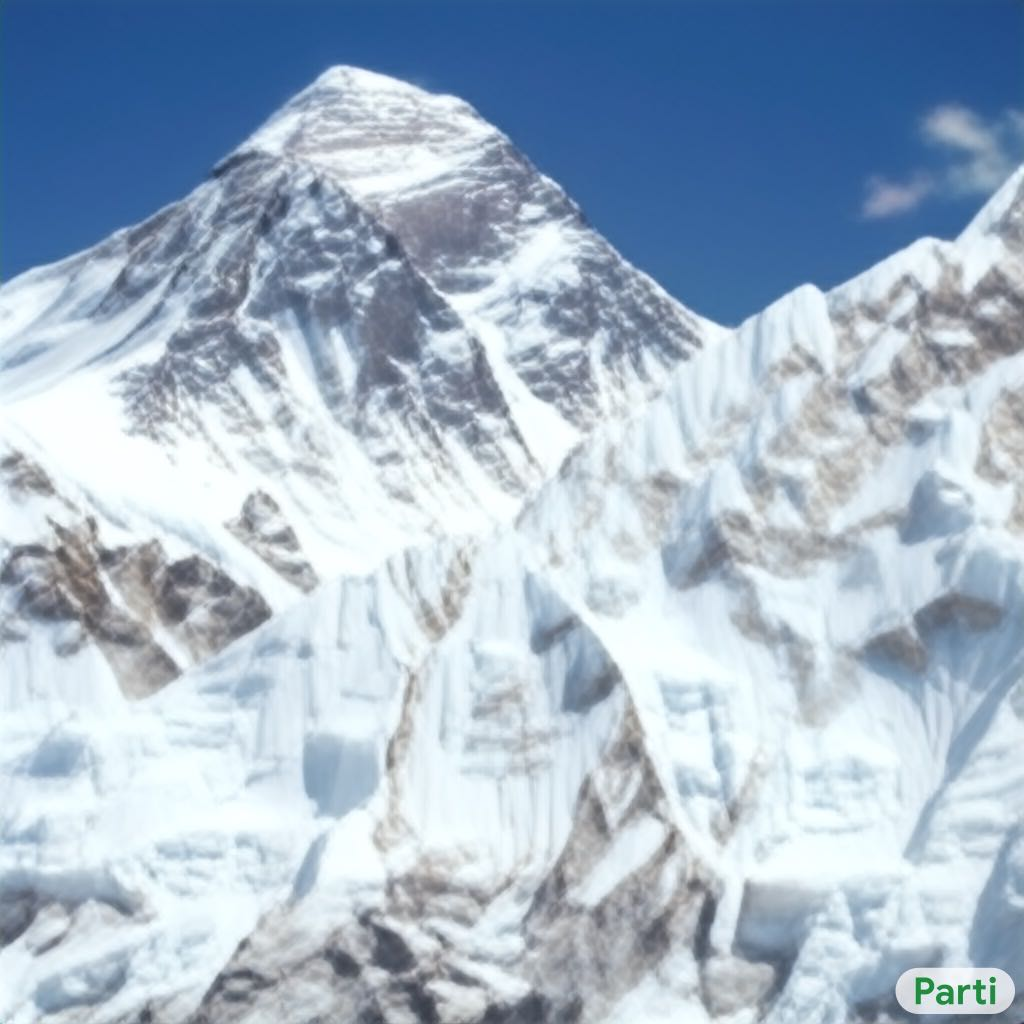
\includegraphics[width=\twobytwocolwidth\textwidth]{figures/limitations/everest_only.jpg}} &
\multicolumn{3}{c}{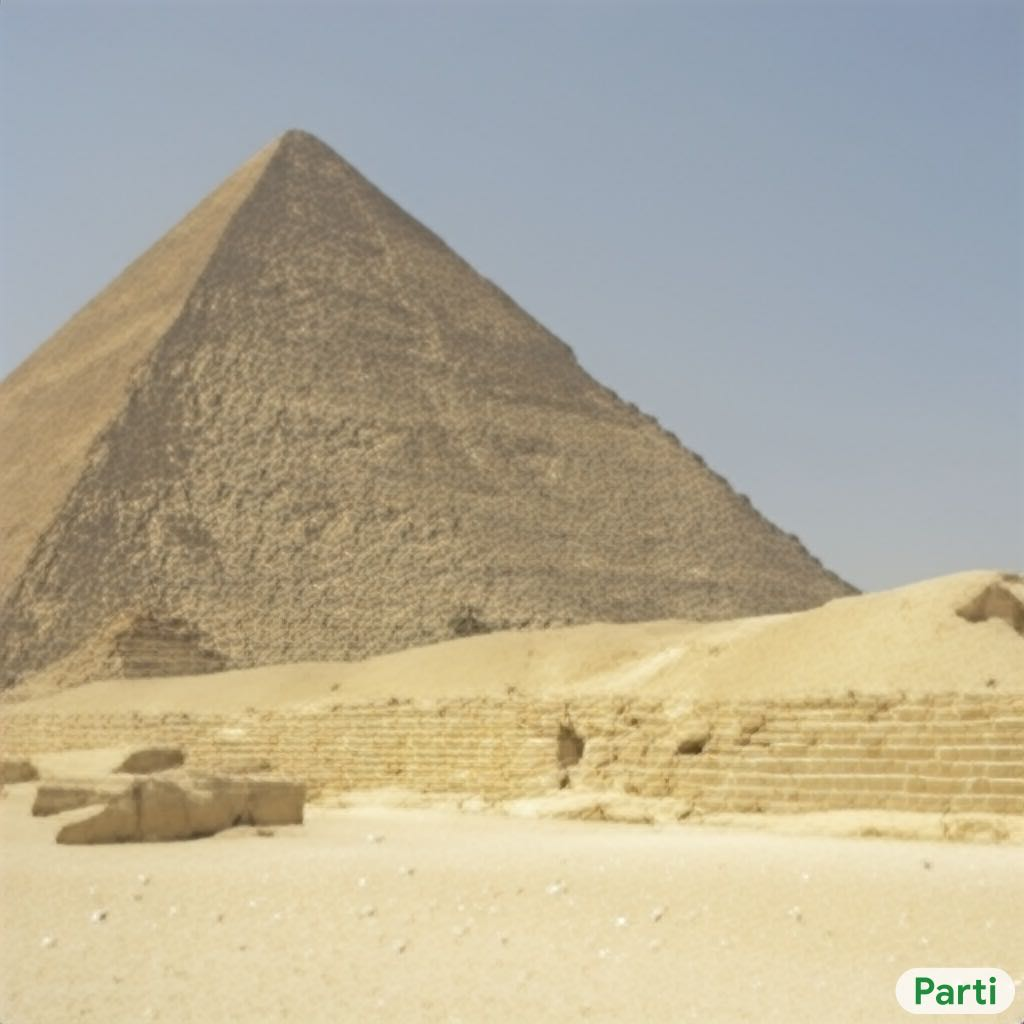
\includegraphics[width=\twobytwocolwidth\textwidth]{figures/limitations/pyramid_only.jpg}} &&
\multicolumn{3}{c}{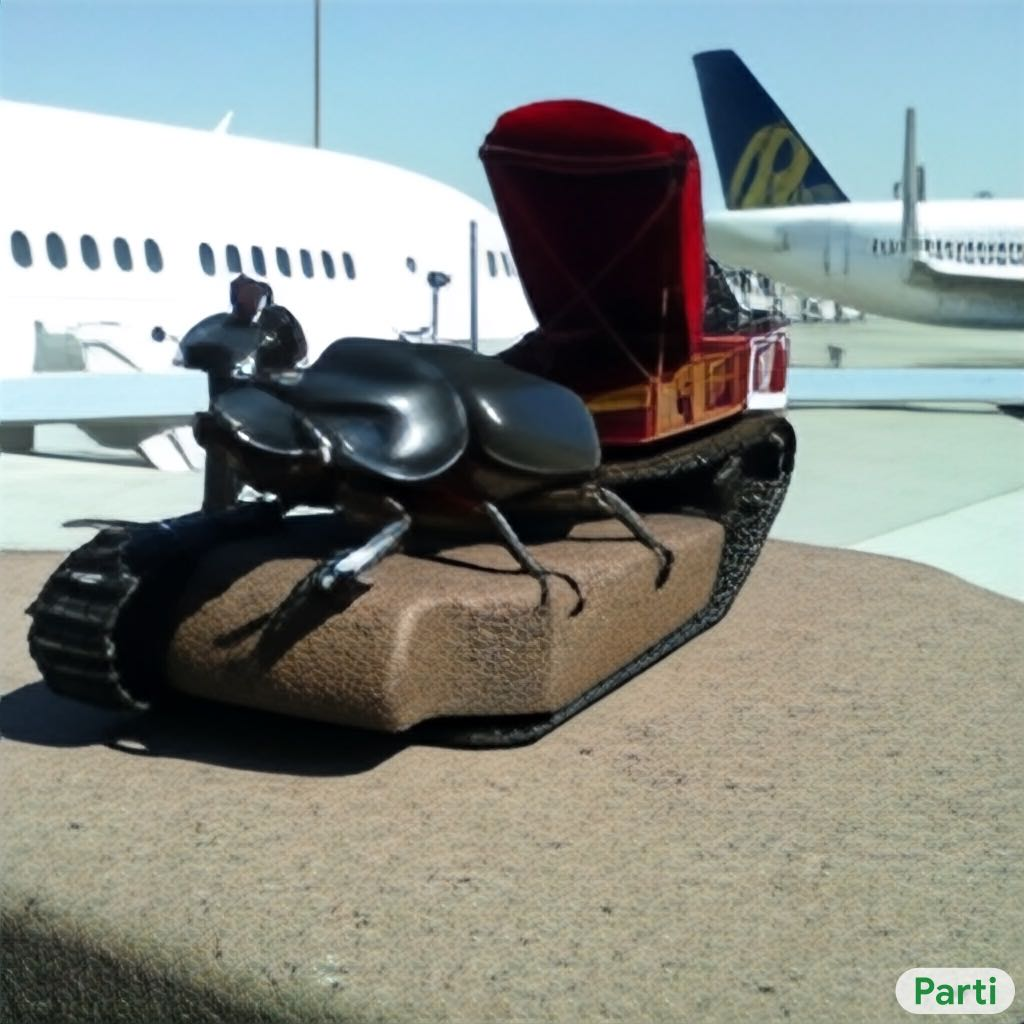
\includegraphics[width=\twobytwocolwidth\textwidth]{figures/limitations/rhino1.jpg}} &
\multicolumn{3}{c}{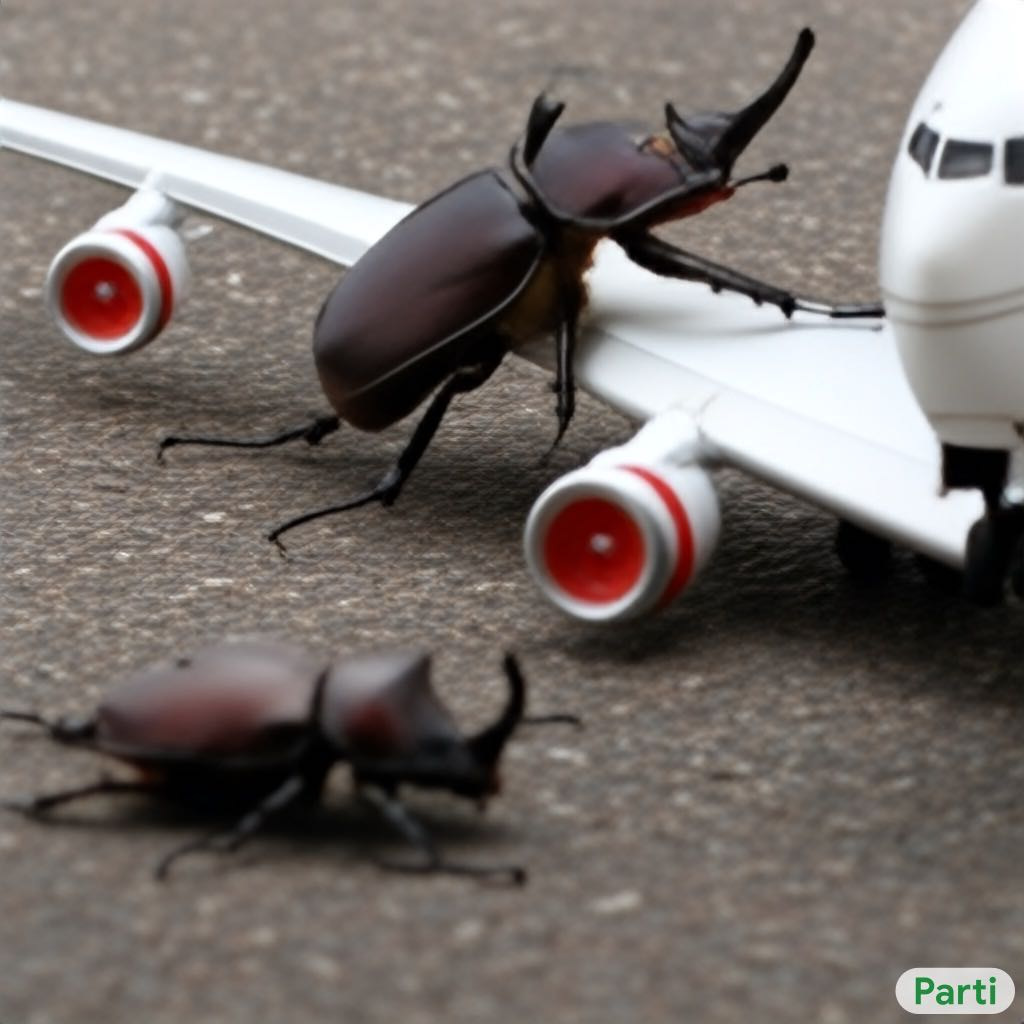
\includegraphics[width=\twobytwocolwidth\textwidth]{figures/limitations/rhino2.jpg}} \\
\multicolumn{3}{c}{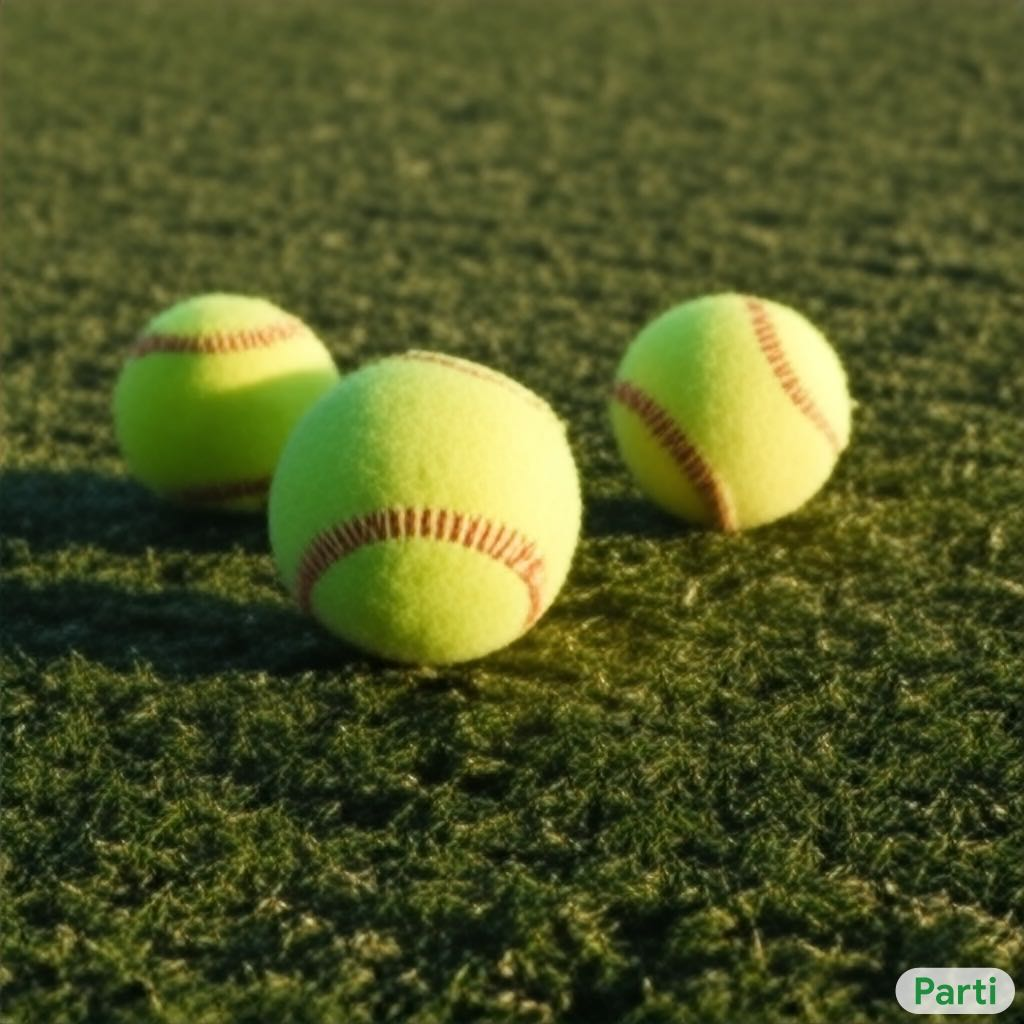
\includegraphics[width=\twobytwocolwidth\textwidth]{figures/limitations/3mergedballs.jpg}} &
\multicolumn{3}{c}{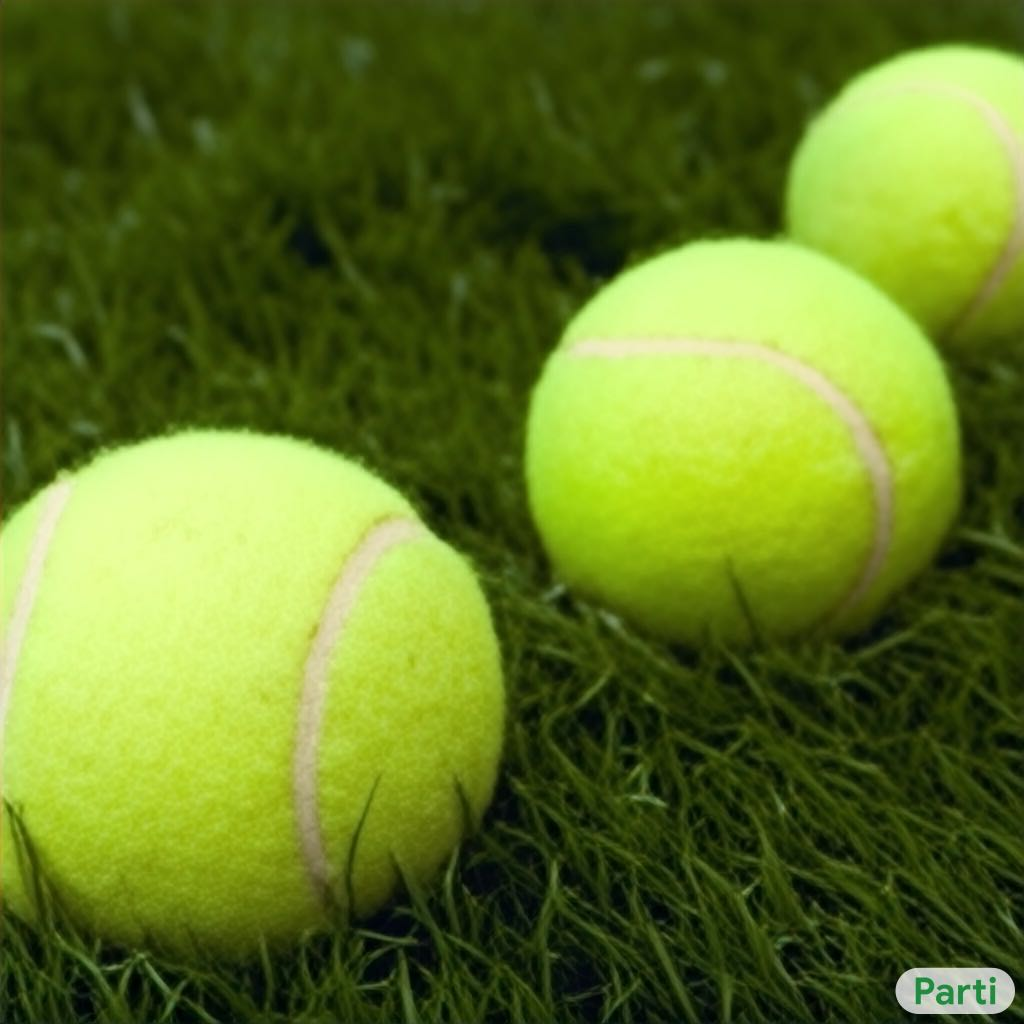
\includegraphics[width=\twobytwocolwidth\textwidth]{figures/limitations/3tennisballs.jpg}} &&
\multicolumn{3}{c}{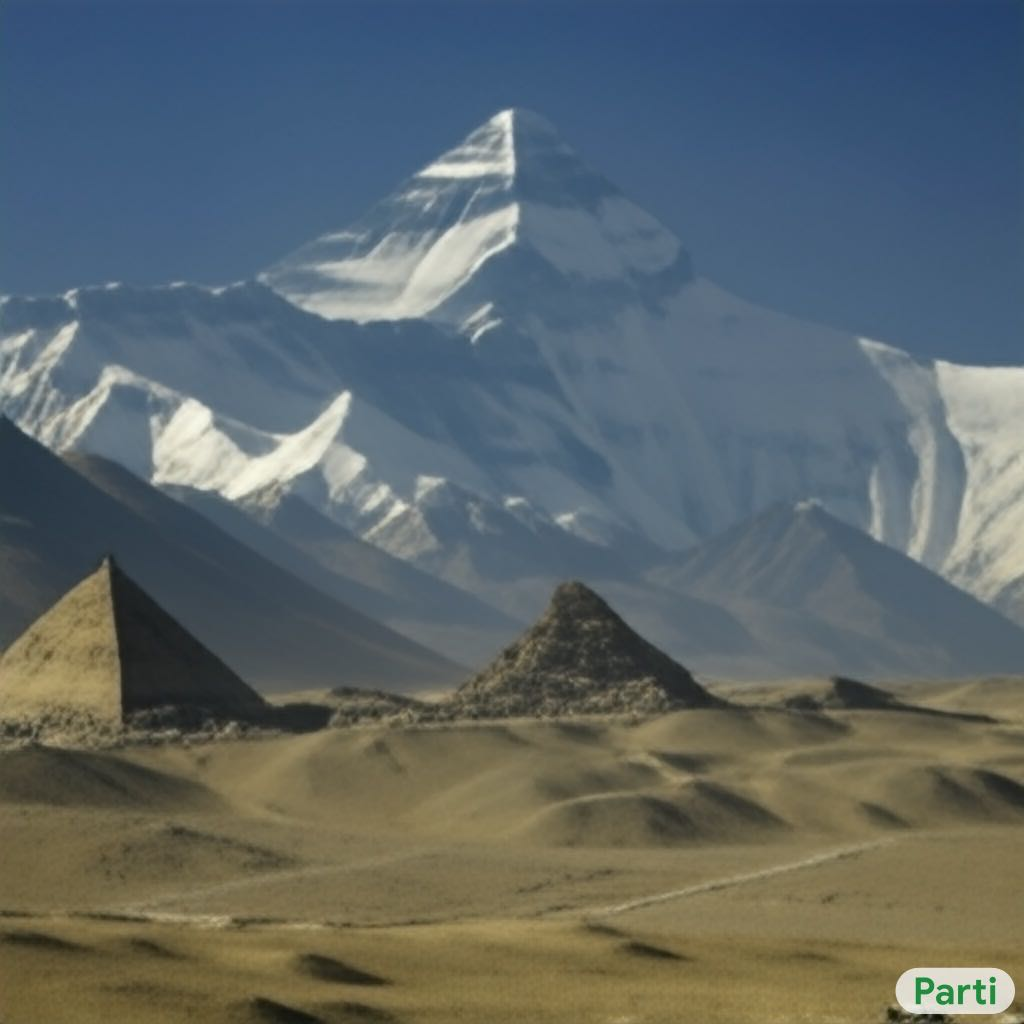
\includegraphics[width=\twobytwocolwidth\textwidth]{figures/limitations/everent_pyramid_merge1.jpg}} &
\multicolumn{3}{c}{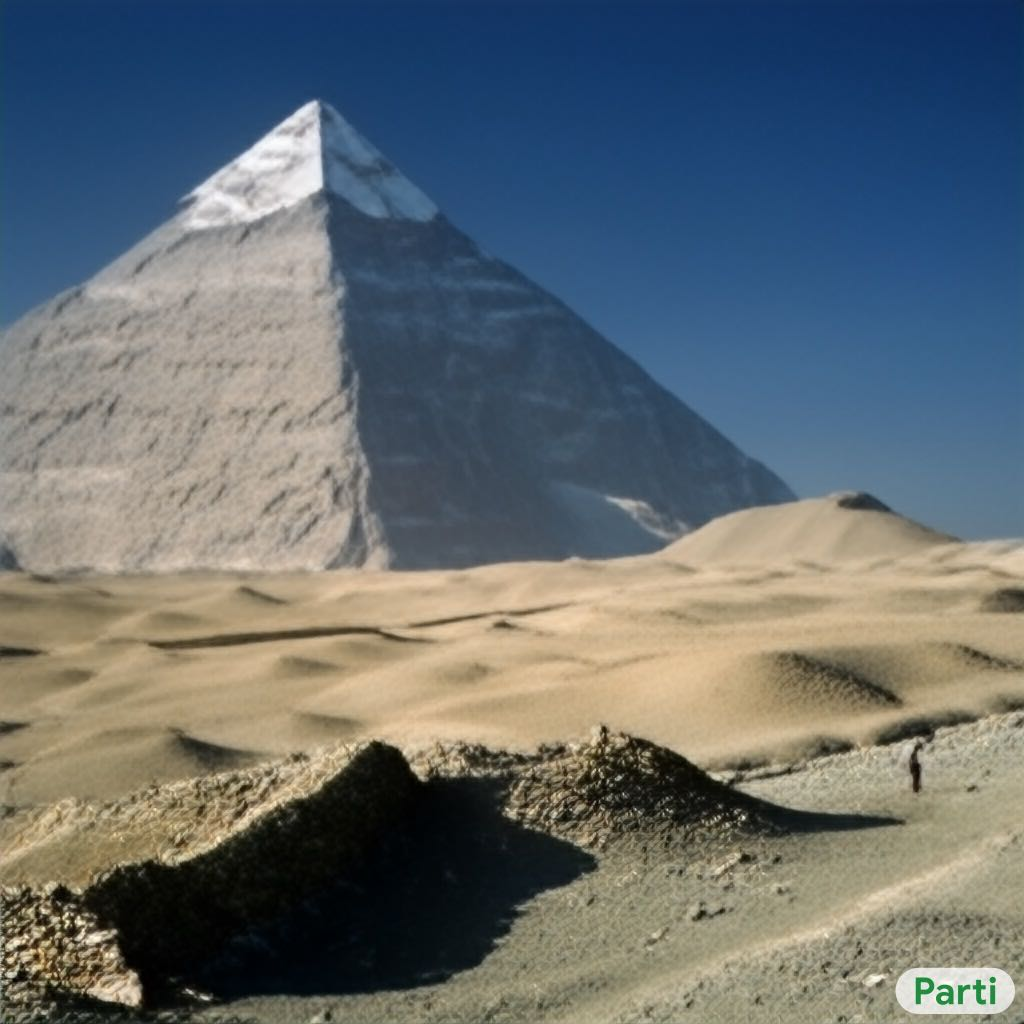
\includegraphics[width=\twobytwocolwidth\textwidth]{figures/limitations/everest_pyramid_merge2.jpg}} &&
\multicolumn{3}{c}{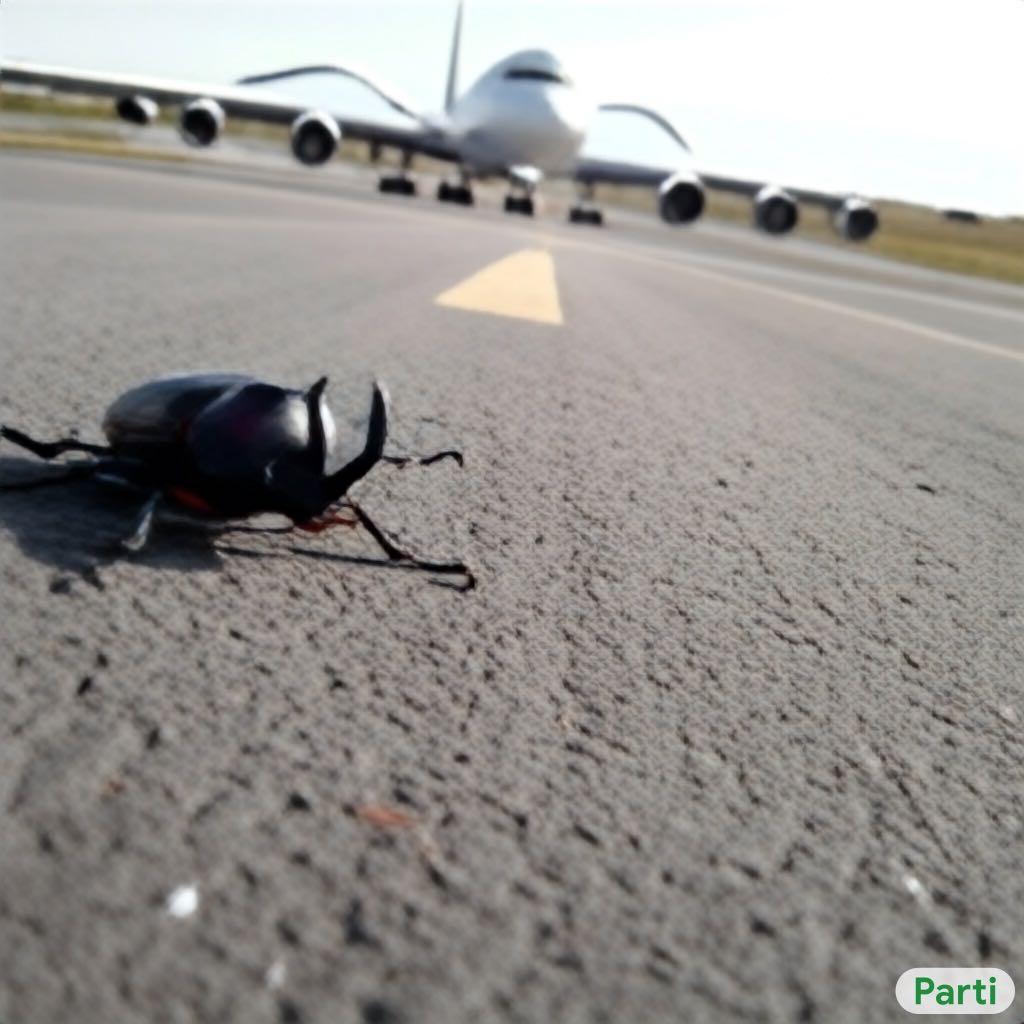
\includegraphics[width=\twobytwocolwidth\textwidth]{figures/limitations/rhino3.jpg}} &
\multicolumn{3}{c}{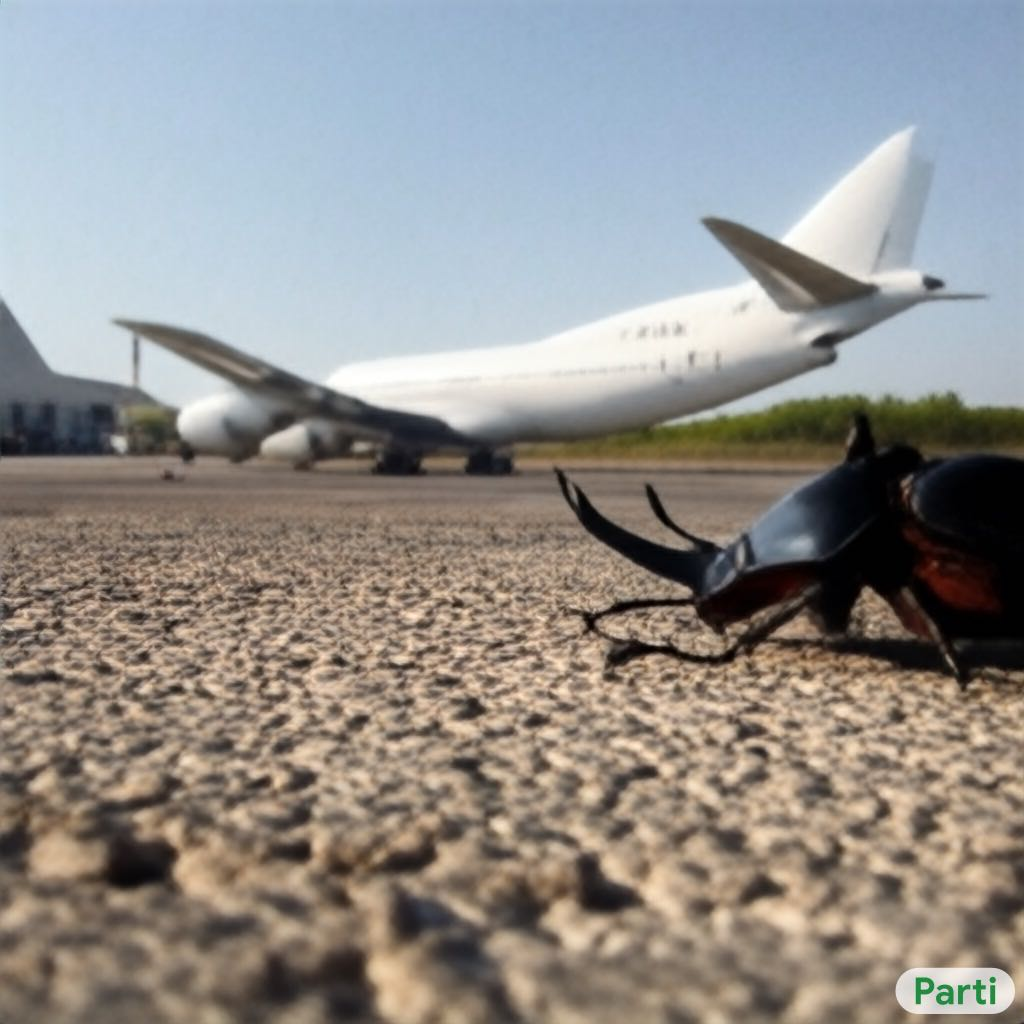
\includegraphics[width=\twobytwocolwidth\textwidth]{figures/limitations/rhino4.jpg}} \\
\multicolumn{6}{C{\thirdcolwidth\textwidth}}{\tiny \textbf{A}. Four images generated in the same batch for the prompt  \textit{two baseballs to the left of three tennis balls}. \textbf{Failures}: color bleeding (b); feature merging (b,c); counting (a-d); spatial relations (a-d). (b-d) also include (arguably reasonable) hallucination of ground details such as gravel and grass.} && 
\multicolumn{6}{C{\thirdcolwidth\textwidth}}{\tiny \textbf{B}. Generated images of (a) \textit{Mount Everest} and (b) \textit{The Great Pyramid} as references and demonstrating the model's knowledge. Two images (c,d) generated for \textit{The Great Pyramid of Giza situated in front of Mount Everest.} \textbf{Failures}: feature-merging of pyramid with pyramidal top of Everest (d) or making a snowy Egyptian Pyramid (d); the pyramid depicted is Khafre's, not Khufu's (Great) Pyramid (d).} && 
\multicolumn{6}{C{\thirdcolwidth\textwidth}}{\tiny \textbf{C}. Four images generated in the same batch for the prompt  \textit{A rhino beetle this size of a tank grapples a real life passenger airplane on the tarmac.} \textbf{Failures}: difficulty in overriding true life size leads to a big beetle poorly merged with a tank (a); toy airplane (b), attempts to use perspective to make a big beetle (c,d), hallucination of extra beetle (b).} \\

\multicolumn{3}{c}{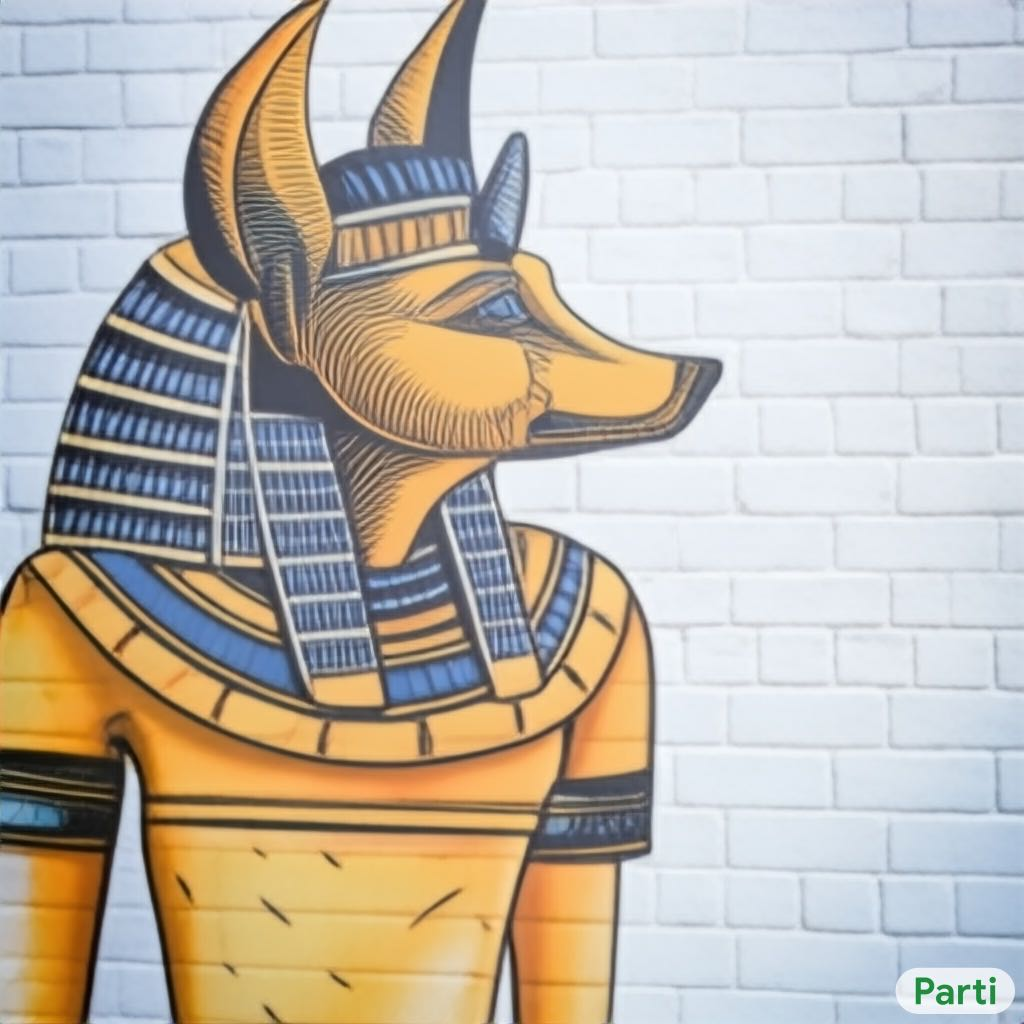
\includegraphics[width=\twobytwocolwidth\textwidth]{figures/limitations/yellow_anubis1.jpg}} &
\multicolumn{3}{c}{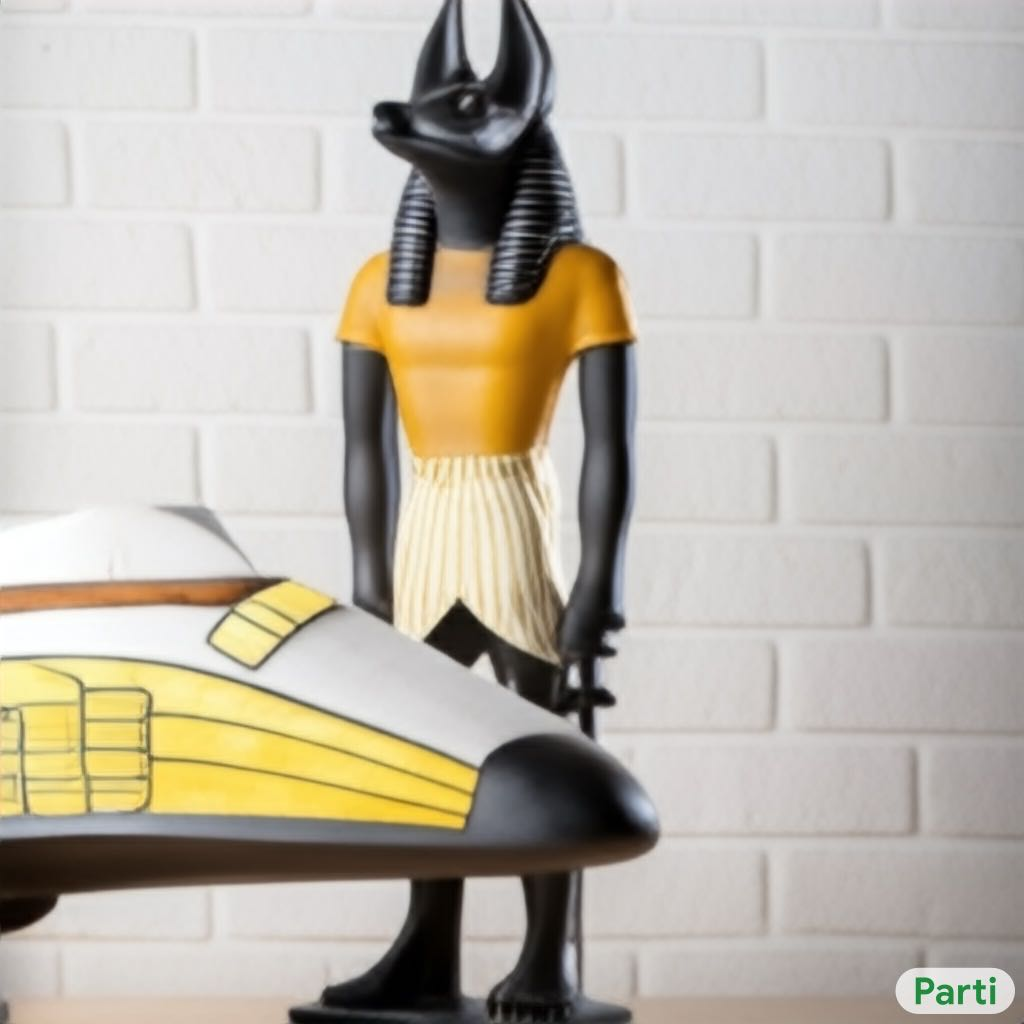
\includegraphics[width=\twobytwocolwidth\textwidth]{figures/limitations/yellow_anubis2.jpg}} &&
\multicolumn{3}{c}{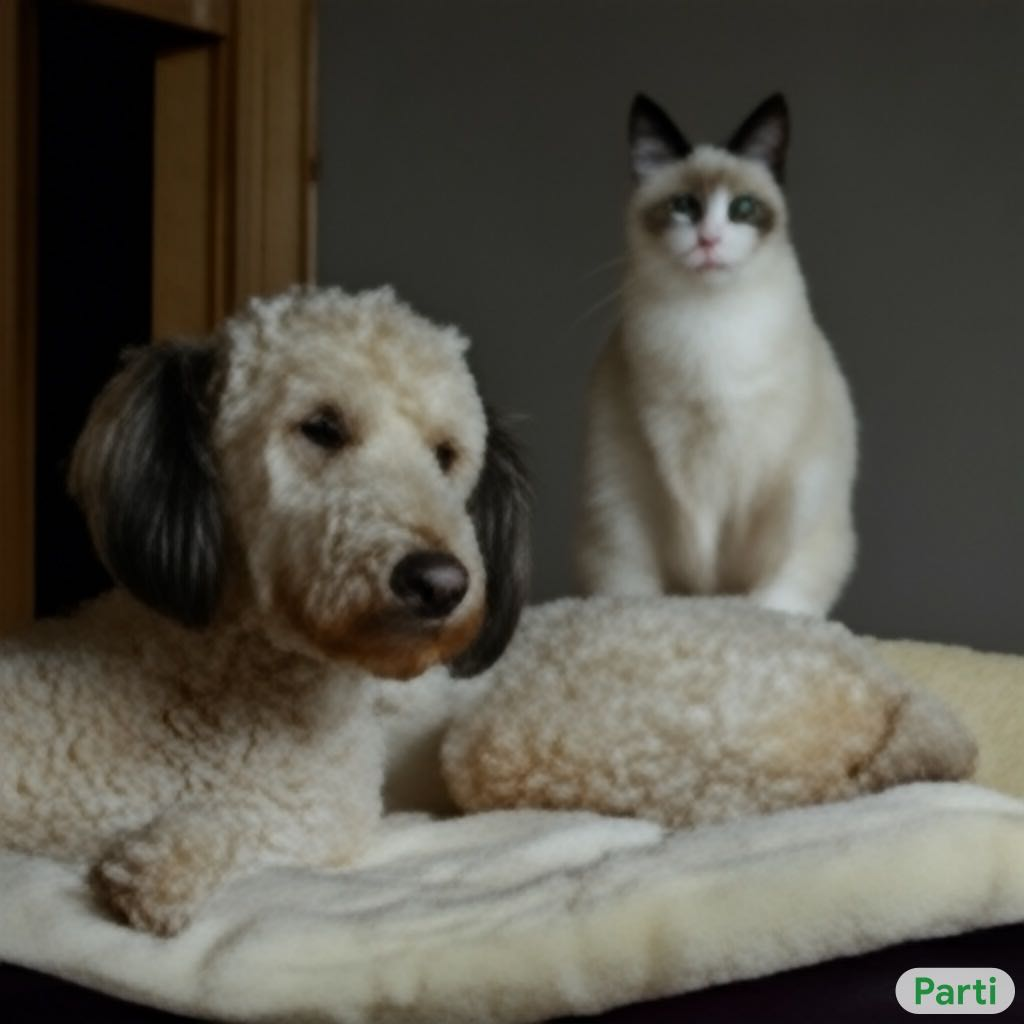
\includegraphics[width=\twobytwocolwidth\textwidth]{figures/limitations/labra_cat1.jpg}} &
\multicolumn{3}{c}{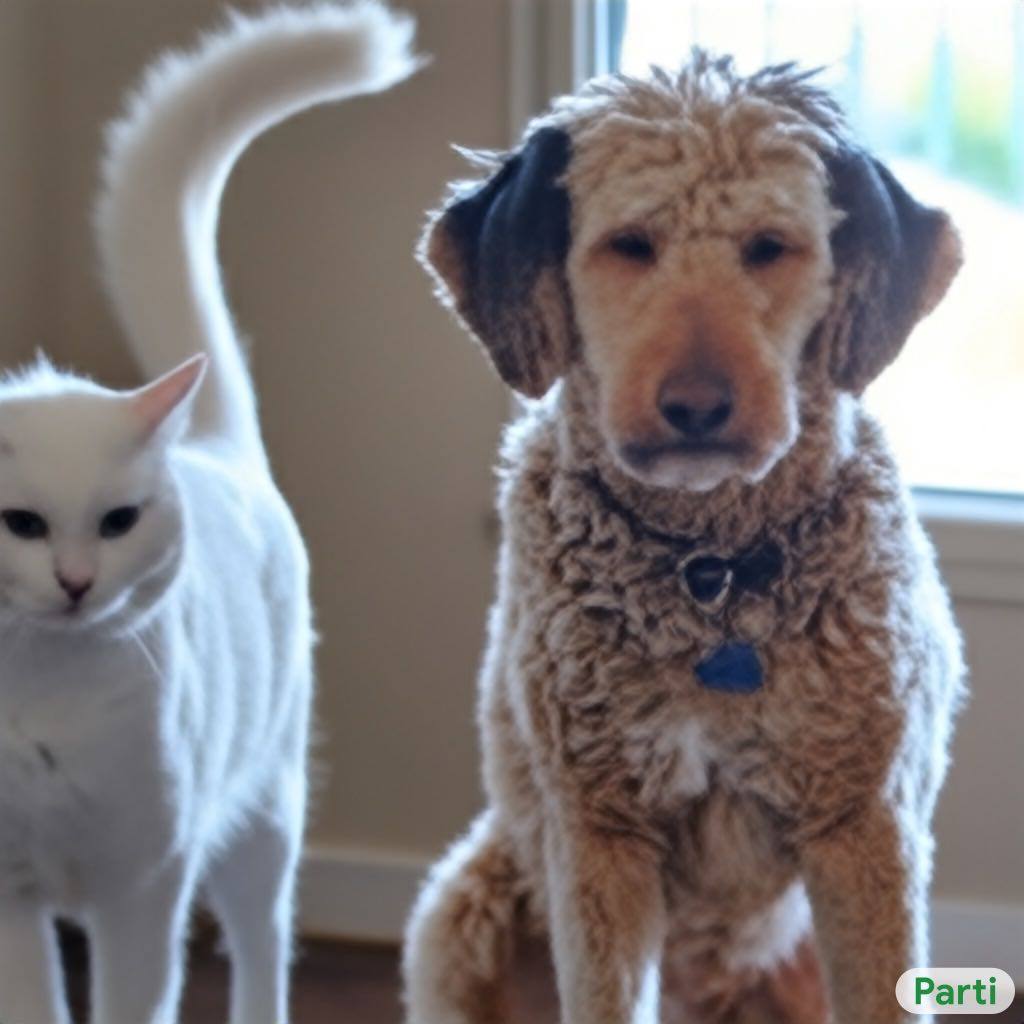
\includegraphics[width=\twobytwocolwidth\textwidth]{figures/limitations/labra_cat4.jpg}} &&
\multicolumn{3}{c}{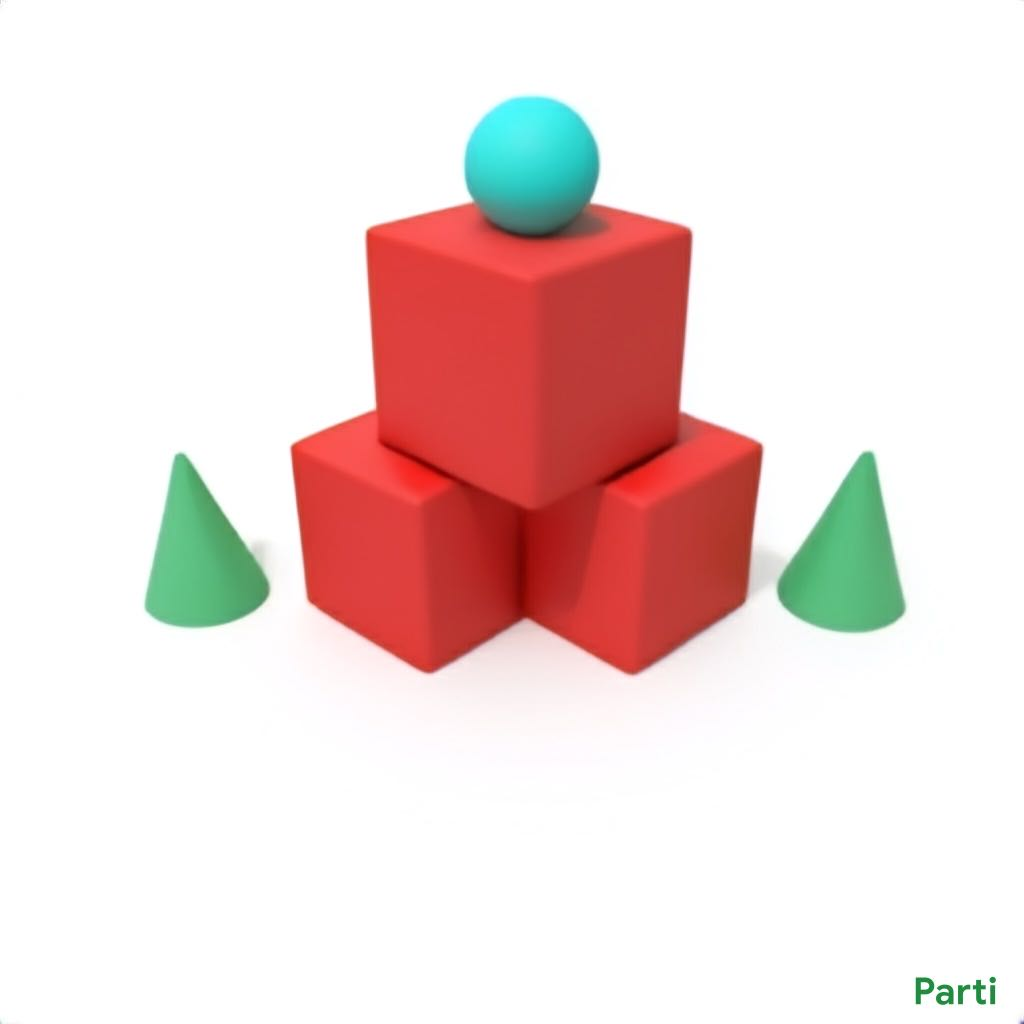
\includegraphics[width=\twobytwocolwidth\textwidth]{figures/limitations/cube_cone1.jpg}} &
\multicolumn{3}{c}{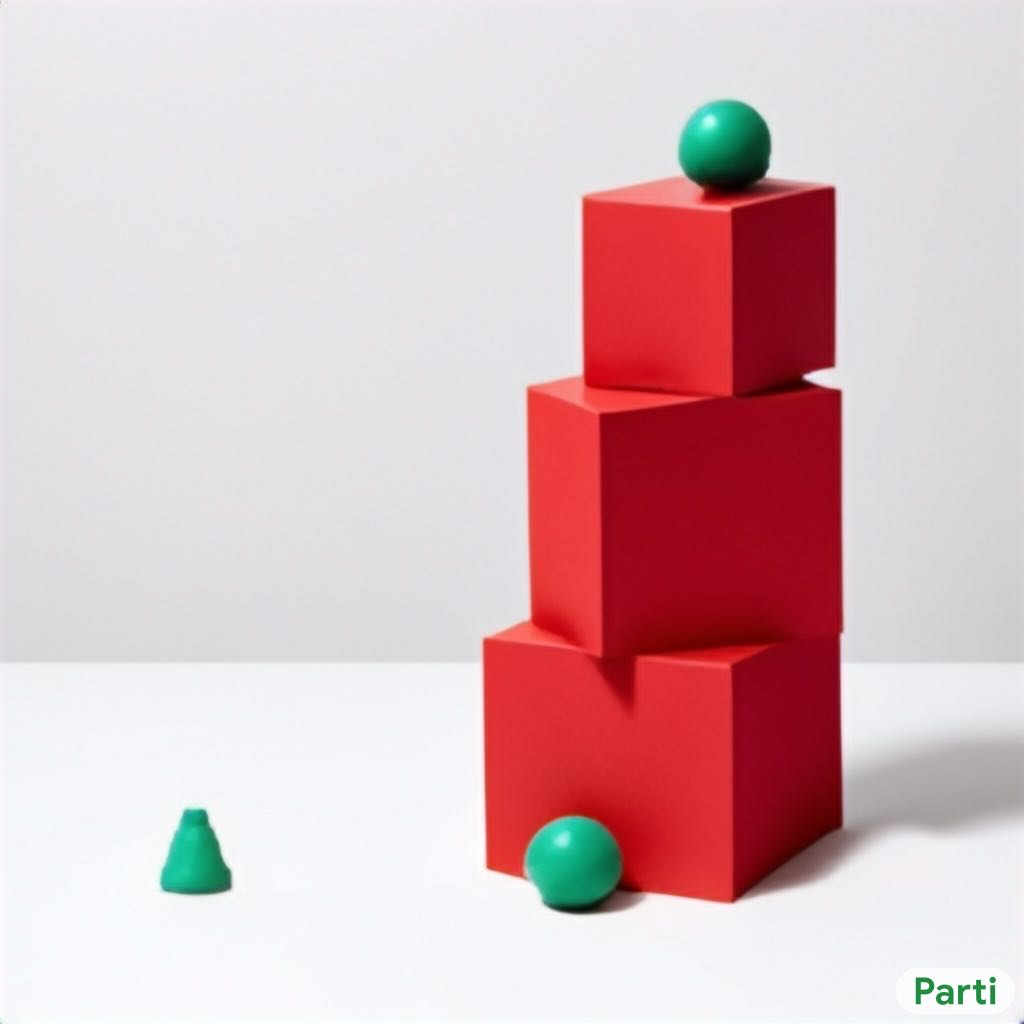
\includegraphics[width=\twobytwocolwidth\textwidth]{figures/limitations/cube_cone2.jpg}} \\
\multicolumn{3}{c}{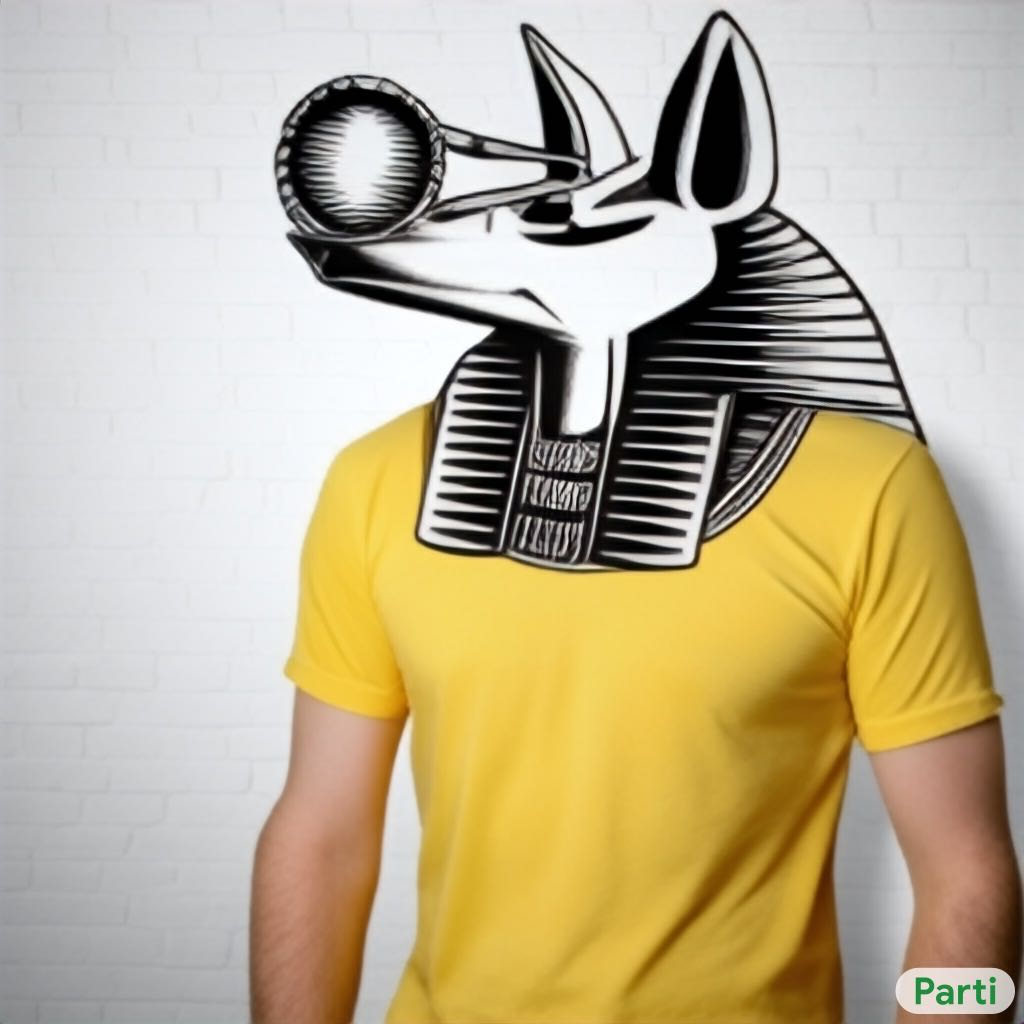
\includegraphics[width=\twobytwocolwidth\textwidth]{figures/limitations/yellow_anubis3.jpg}} &
\multicolumn{3}{c}{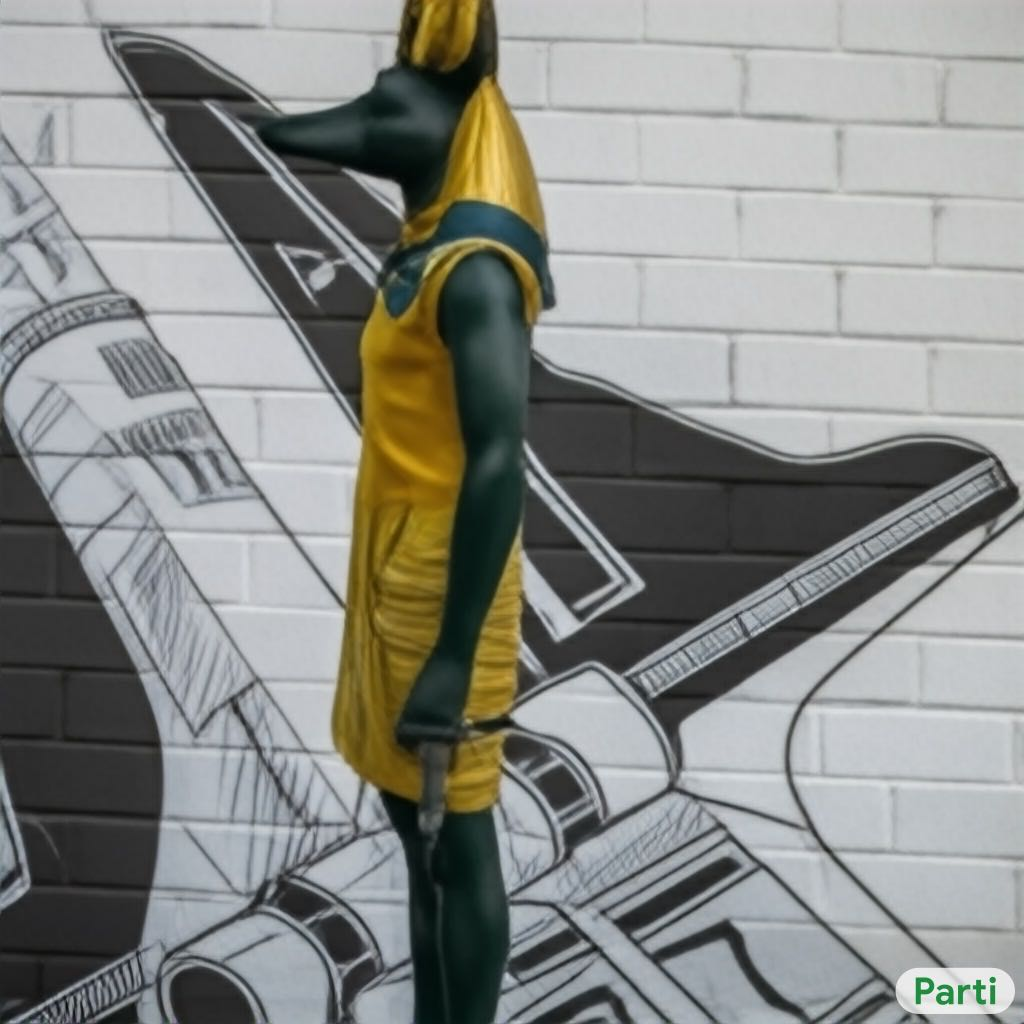
\includegraphics[width=\twobytwocolwidth\textwidth]{figures/limitations/yellow_anubis4.jpg}} &&
\multicolumn{3}{c}{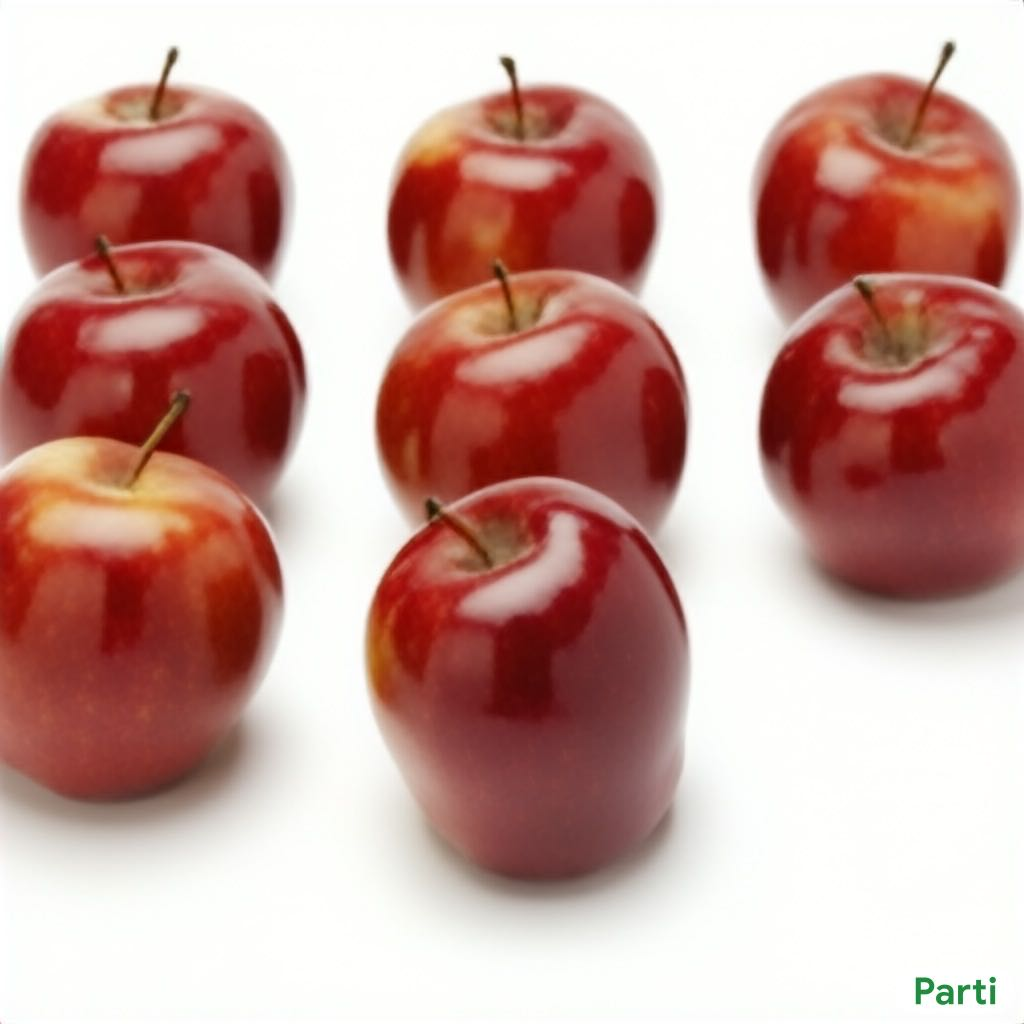
\includegraphics[width=\twobytwocolwidth\textwidth]{figures/limitations/apples_count8.jpg}} &
\multicolumn{3}{c}{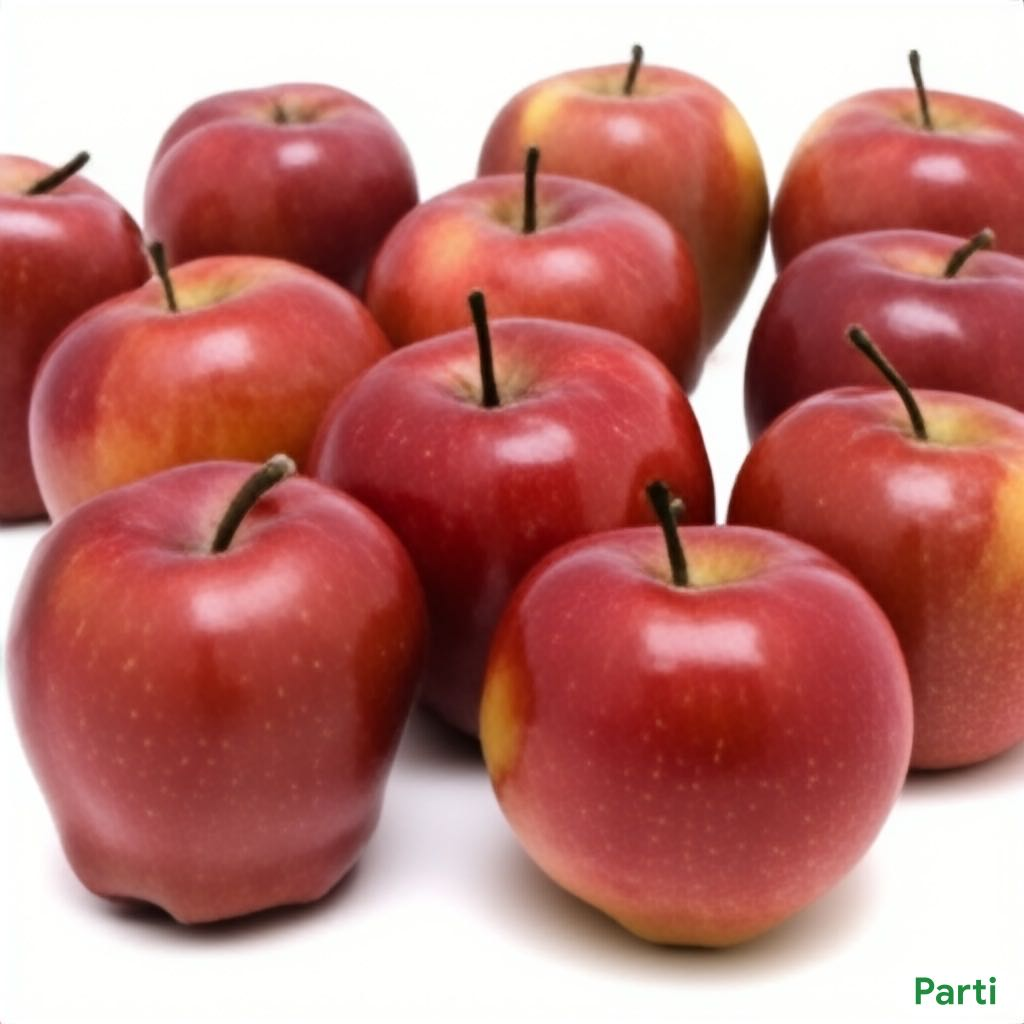
\includegraphics[width=\twobytwocolwidth\textwidth]{figures/limitations/apples_count11.jpg}} &&
\multicolumn{3}{c}{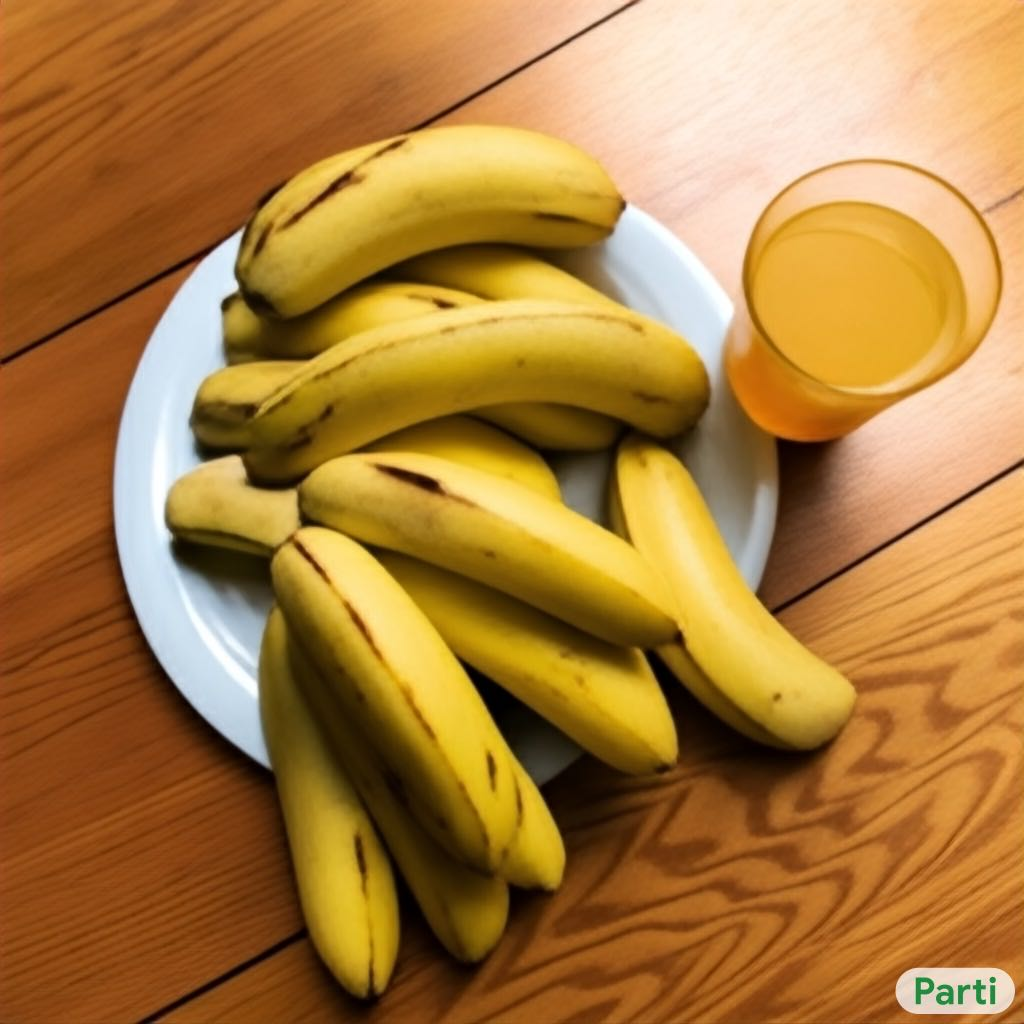
\includegraphics[width=\twobytwocolwidth\textwidth]{figures/limitations/banana_juice_1.jpg}} &
\multicolumn{3}{c}{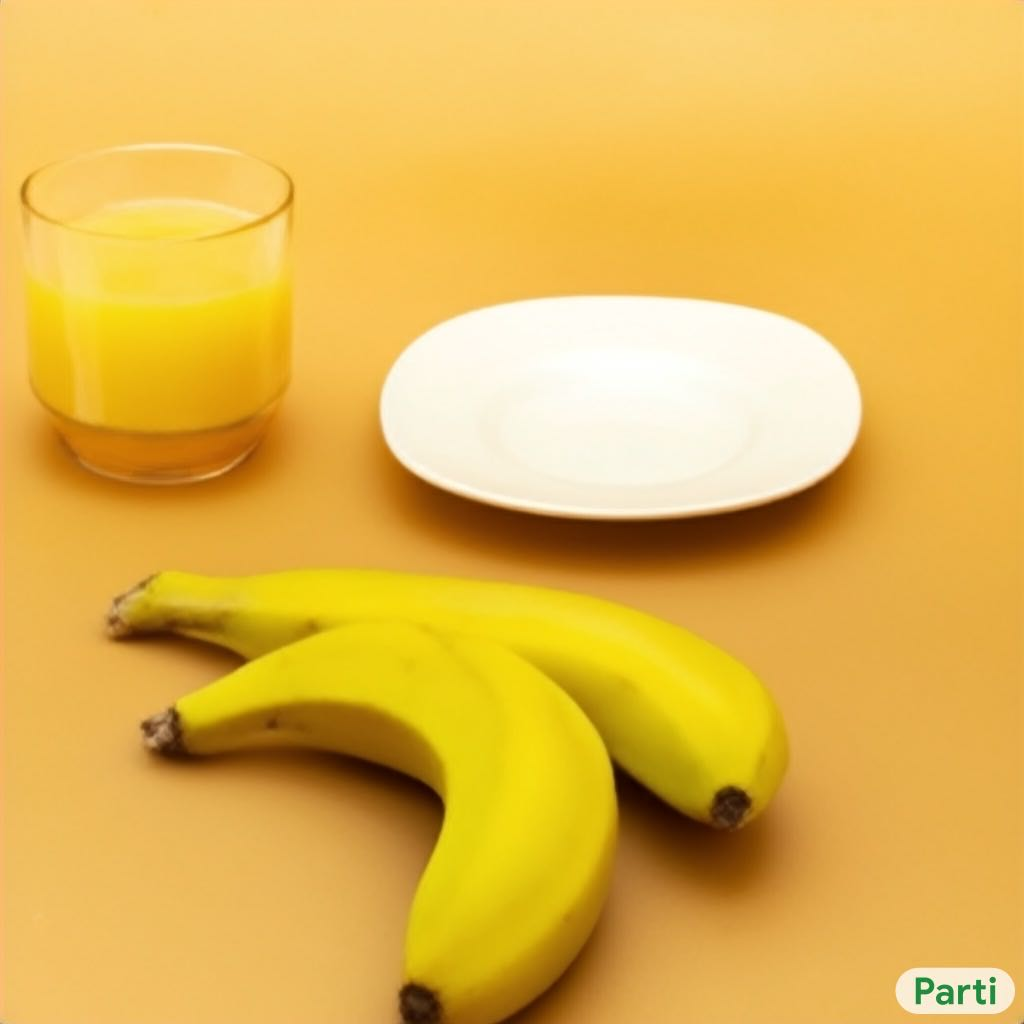
\includegraphics[width=\twobytwocolwidth\textwidth]{figures/limitations/banana_juice_2.jpg}} \\
\multicolumn{6}{C{\thirdcolwidth\textwidth}}{\tiny \textbf{D}. Four images generated in the same batch for the prompt  \textit{A portrait of a statue of Anubis with a crown and wearing a yellow t-shirt that has a space shuttle drawn on it. A white brick wall is in the background.} \textbf{Failures}: color bleeding (a,d); incorrect visual aspect (a,b,d); (unspecified) media blending (c); displaced positioning (b,d); missing details (a,c).} && 
\multicolumn{6}{C{\thirdcolwidth\textwidth}}{\tiny \textbf{E}. (a,b) Two images generated in the same batch for  \textit{a cream colored labradoodle next to a white cat with black-tipped ears}. (c,d) Two images generated in the same batch for \textit{ten red apples}. \textbf{Failures}: hard to disentangle specific features assigned to multiple entities in the same description (a,b); incorrect count of 8 (a) and 11 (b). (Note that some correctly had ten apples.)} && 
\multicolumn{6}{C{\thirdcolwidth\textwidth}}{\tiny \textbf{F}. (a, b) Two images in the same batch for the prompt  \textit{a stack of three red cubes with a blue sphere on the right and two green cones on the left}. (c, d) Two images in the same batch for the prompt \textit{a plate that has no bananas on it. there is a glass without orange juice next to it.} \textbf{Failures}: Incorrect relative positioning of objects (a,b,d). Incorrect coloring-to-attribute association (b). Hallucination (of objects specifically mentioned as absent) (c, d).} \\

\multicolumn{3}{c}{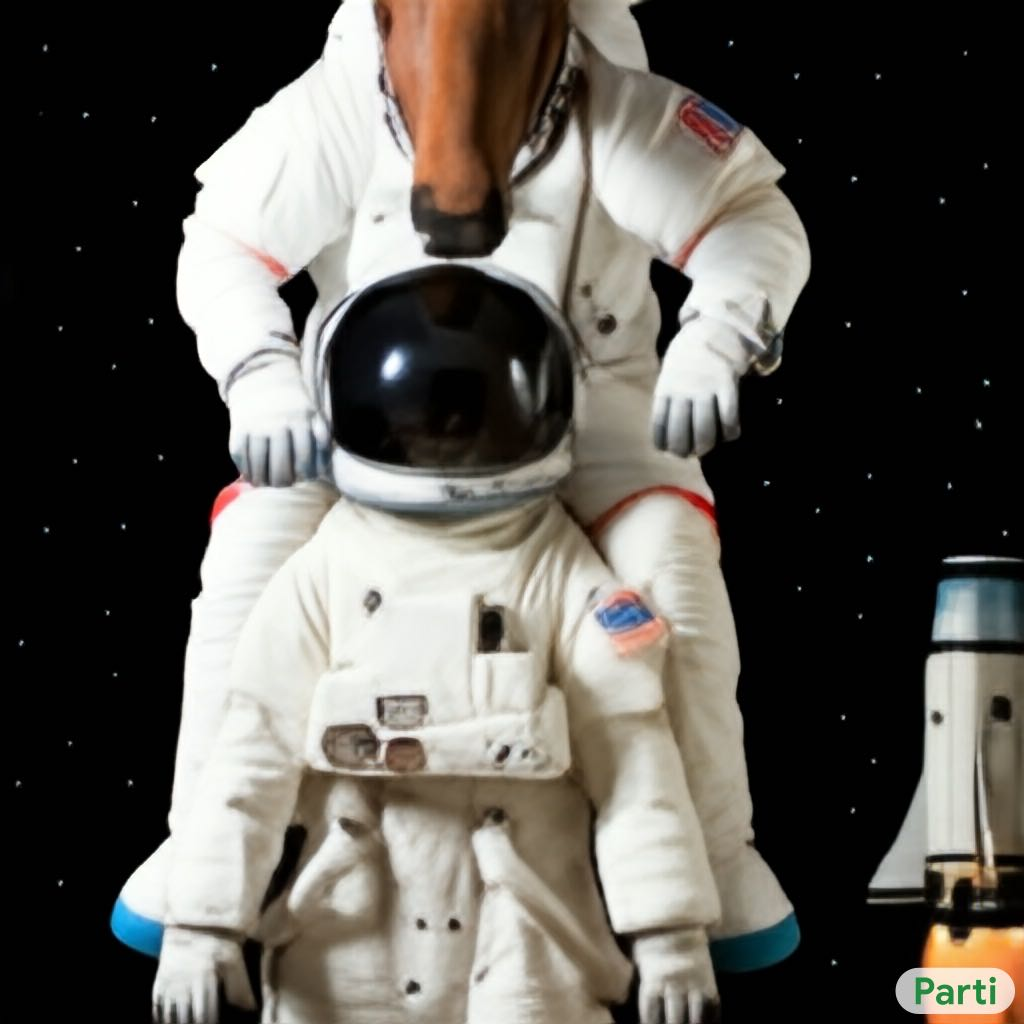
\includegraphics[width=\twobytwocolwidth\textwidth]{figures/limitations/astrohorse1.jpg}} &
\multicolumn{3}{c}{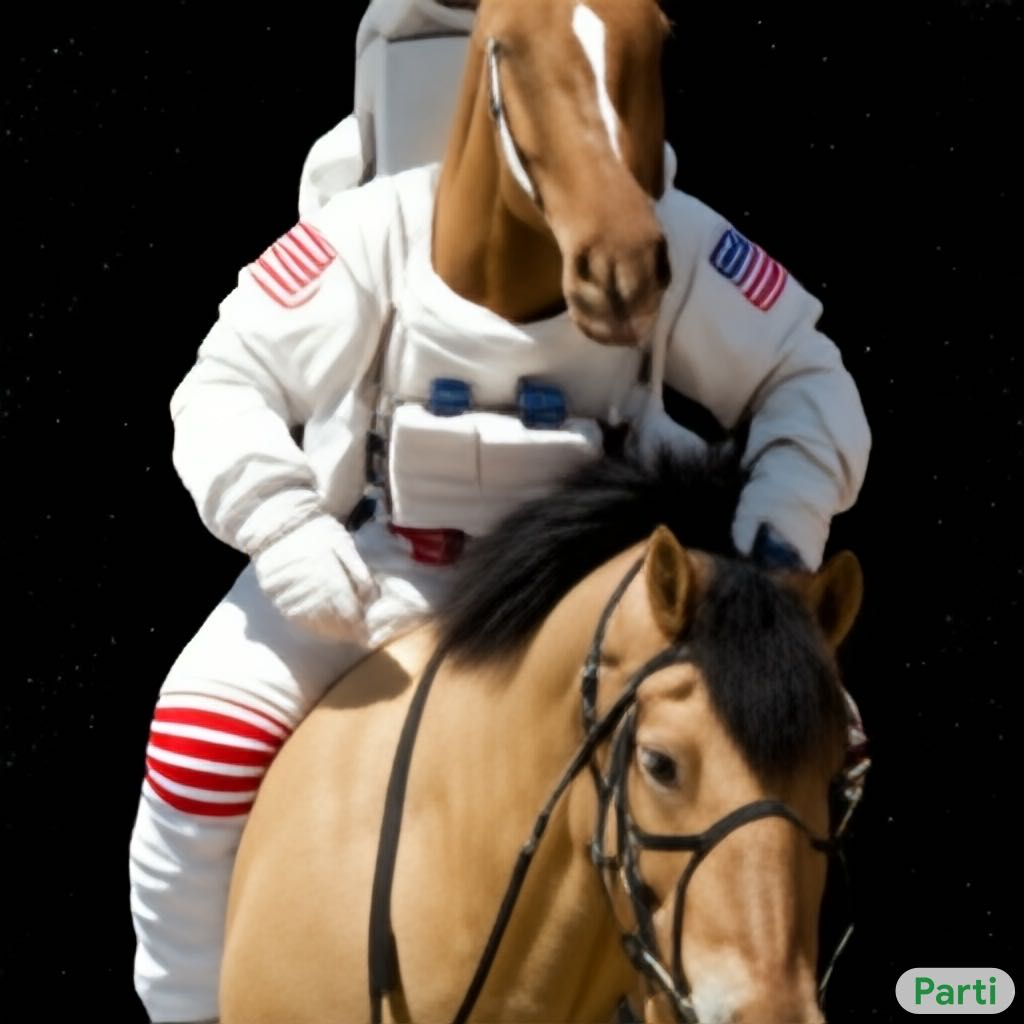
\includegraphics[width=\twobytwocolwidth\textwidth]{figures/limitations/astrohorse2.jpg}} &&
\multicolumn{3}{c}{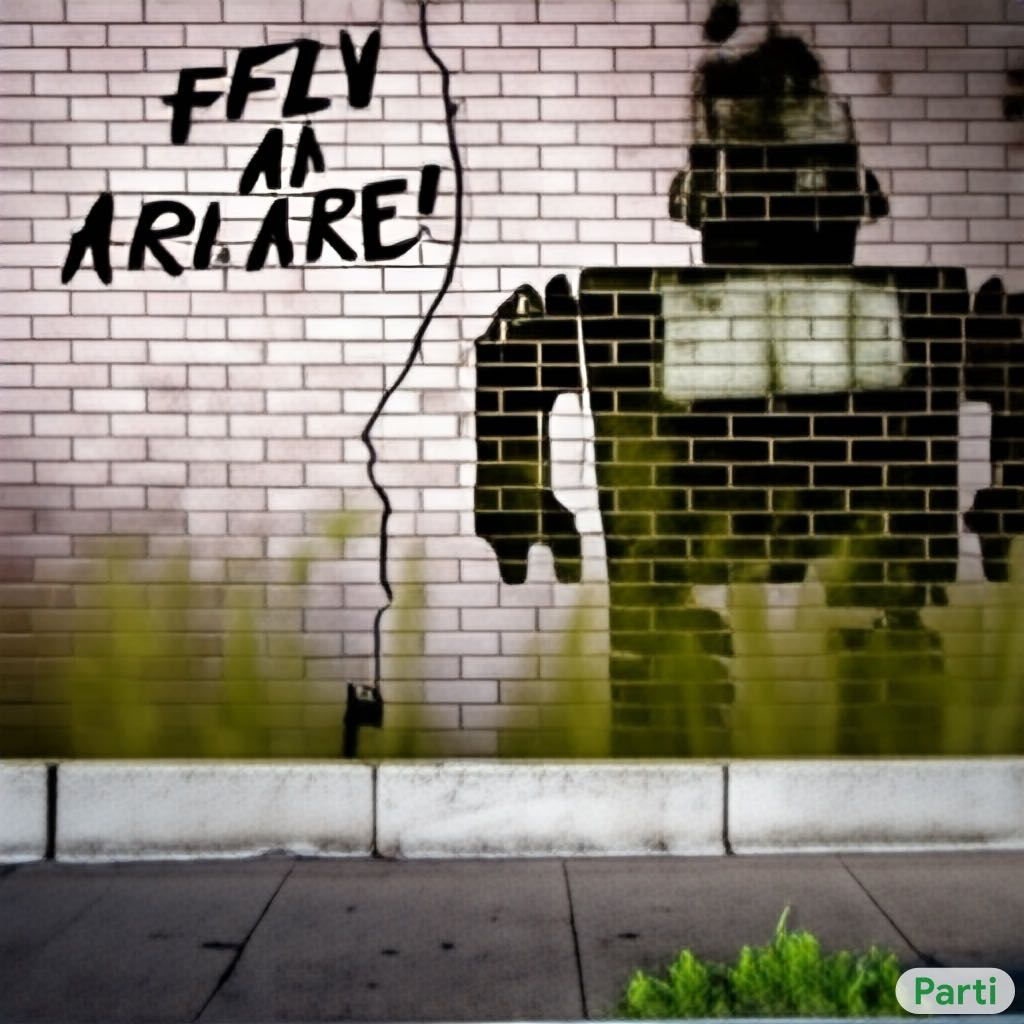
\includegraphics[width=\twobytwocolwidth\textwidth]{figures/limitations/robot_airplane1.jpg}} &
\multicolumn{3}{c}{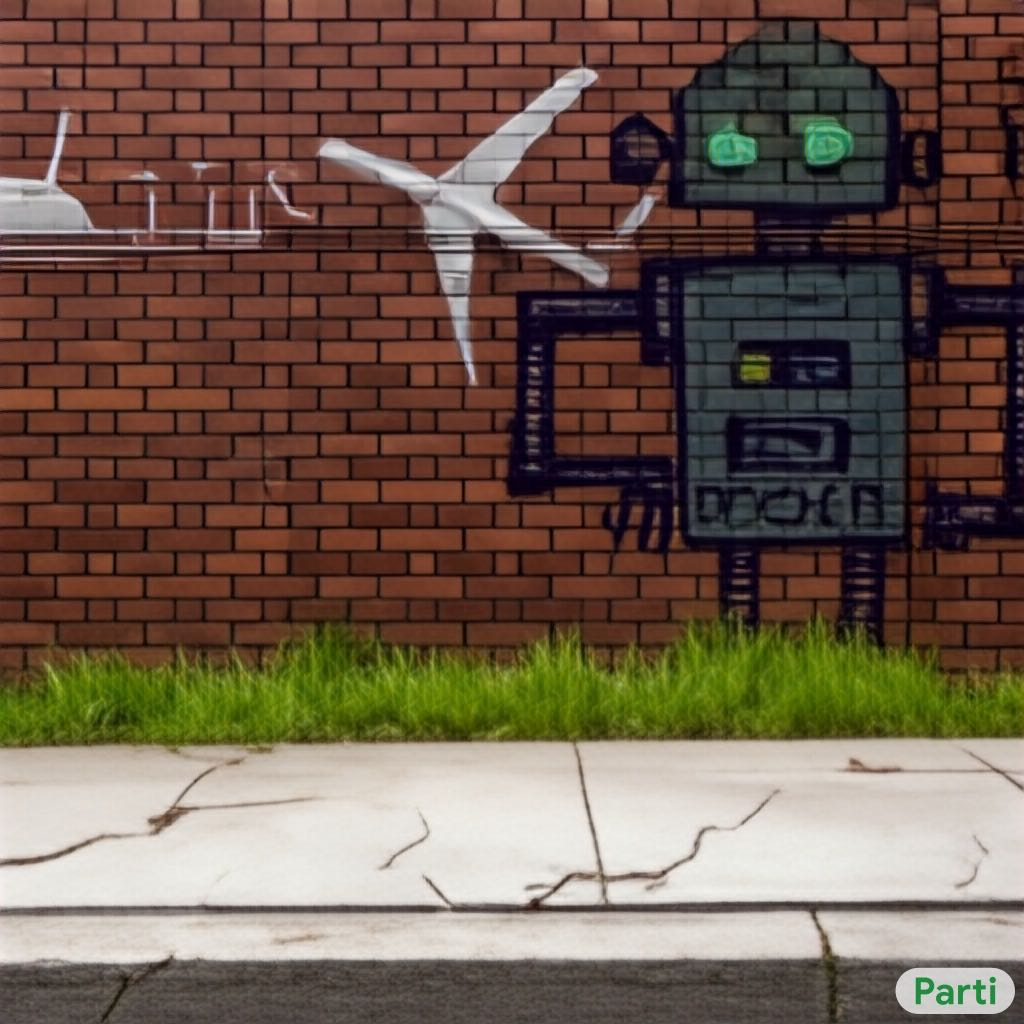
\includegraphics[width=\twobytwocolwidth\textwidth]{figures/limitations/robot_airplane2.jpg}} &&
\multicolumn{3}{c}{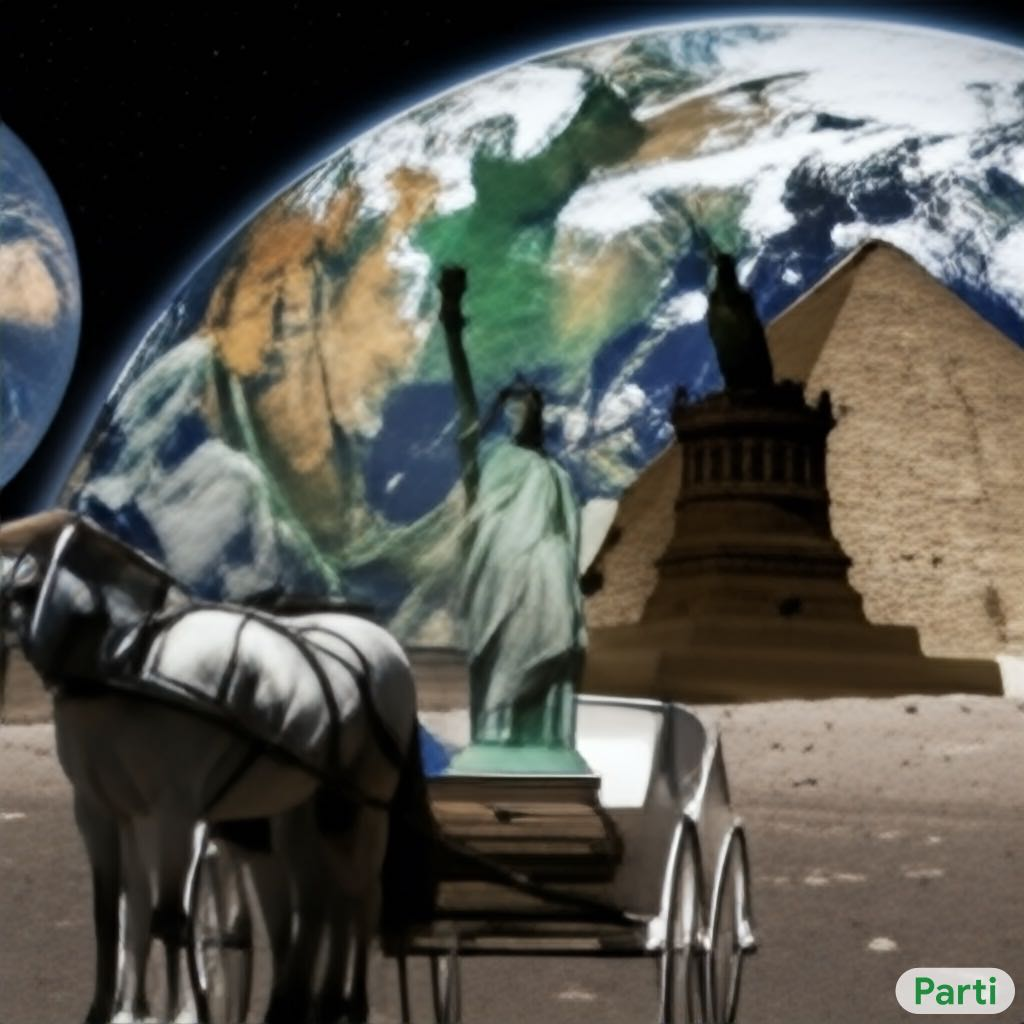
\includegraphics[width=\twobytwocolwidth\textwidth]{figures/limitations/moon_impossible1.jpg}} &
\multicolumn{3}{c}{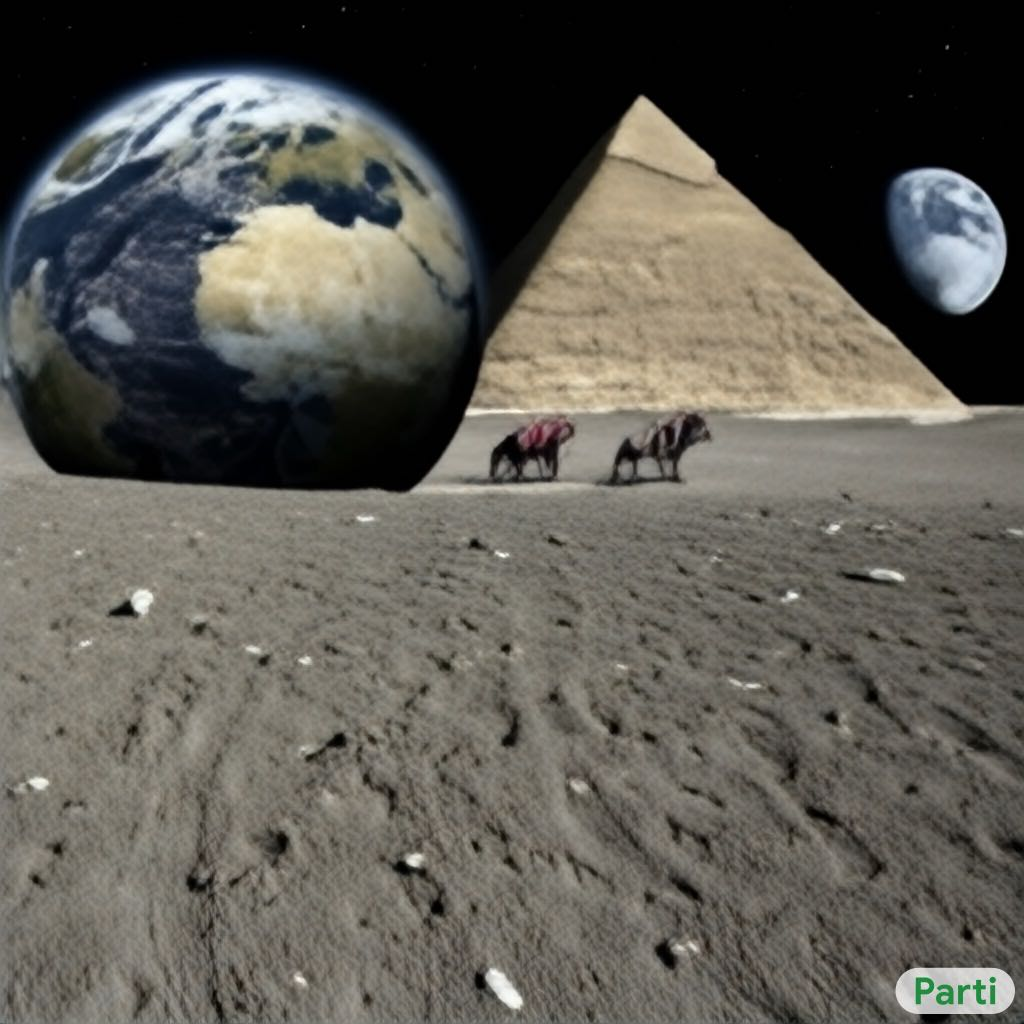
\includegraphics[width=\twobytwocolwidth\textwidth]{figures/limitations/moon_impossible2.jpg}} \\
\multicolumn{3}{c}{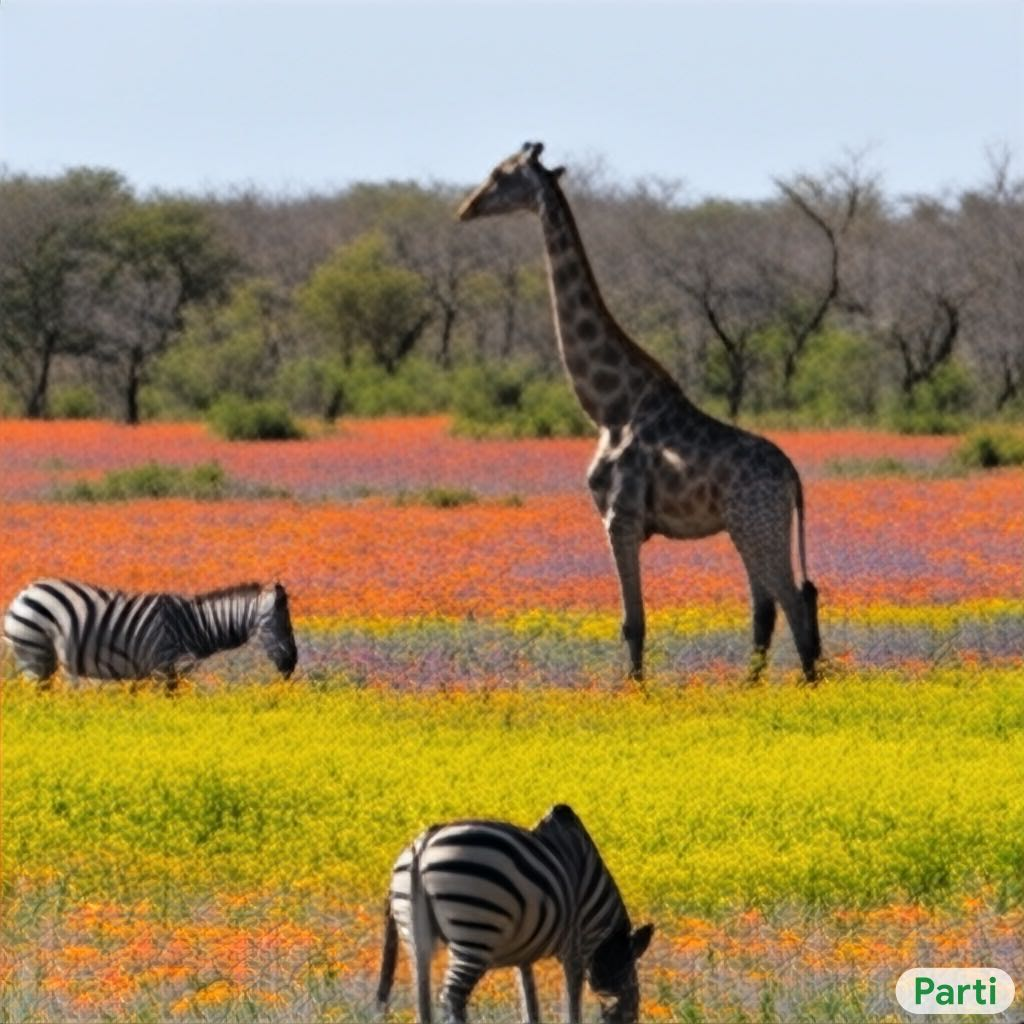
\includegraphics[width=\twobytwocolwidth\textwidth]{figures/limitations/giraffe_zebra3.jpg}} &
\multicolumn{3}{c}{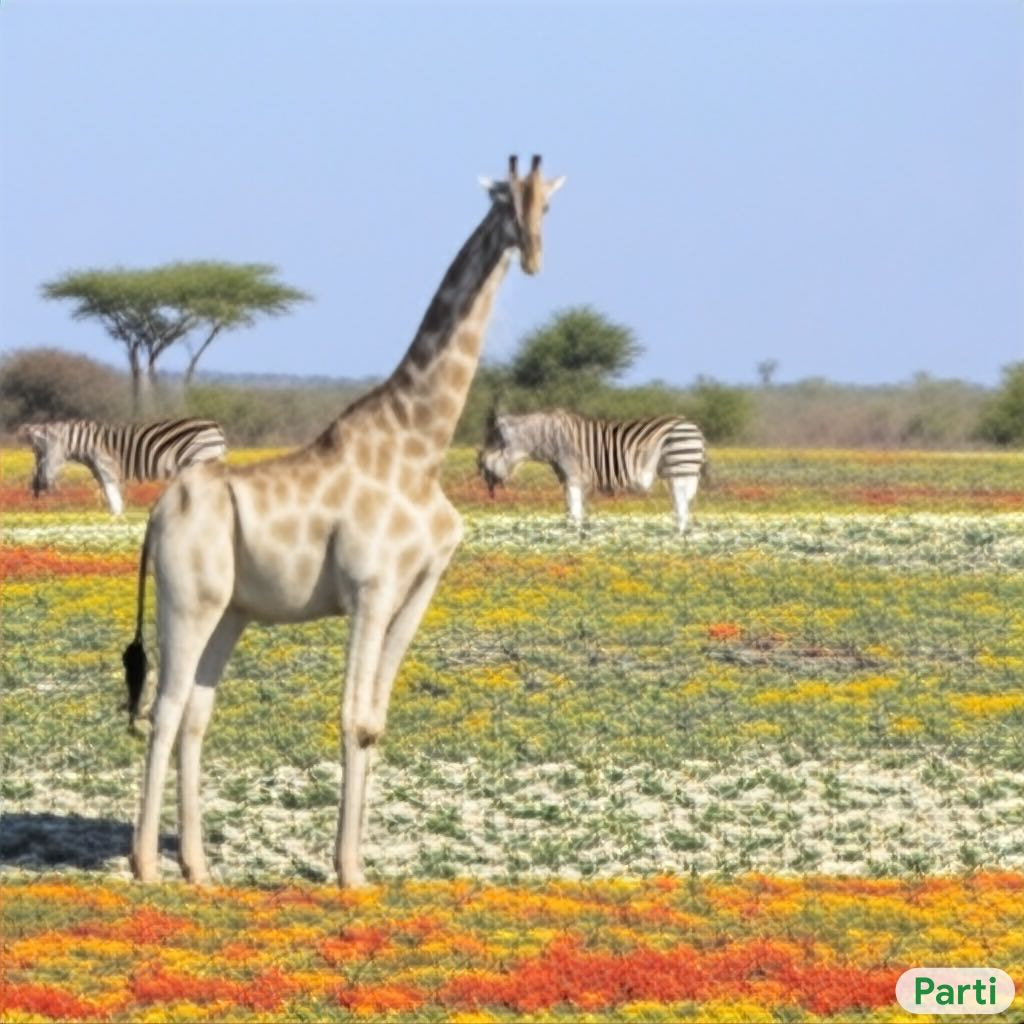
\includegraphics[width=\twobytwocolwidth\textwidth]{figures/limitations/giraffe_zebra4.jpg}} &&
\multicolumn{3}{c}{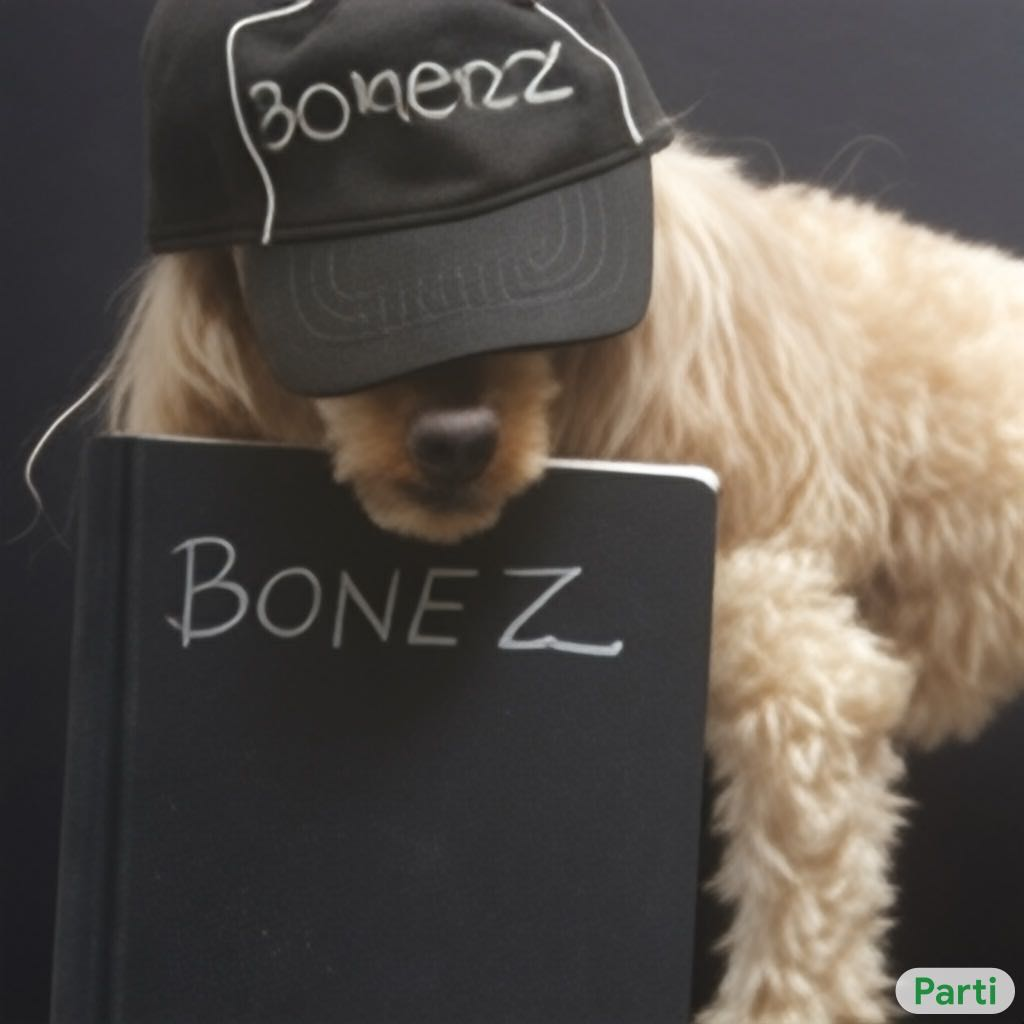
\includegraphics[width=\twobytwocolwidth\textwidth]{figures/limitations/poodle_board3.jpg}} &
\multicolumn{3}{c}{
\includegraphics[width=\twobytwocolwidth\textwidth]{figures/limitations/poodle_board4.jpg}} &&
\multicolumn{3}{c}{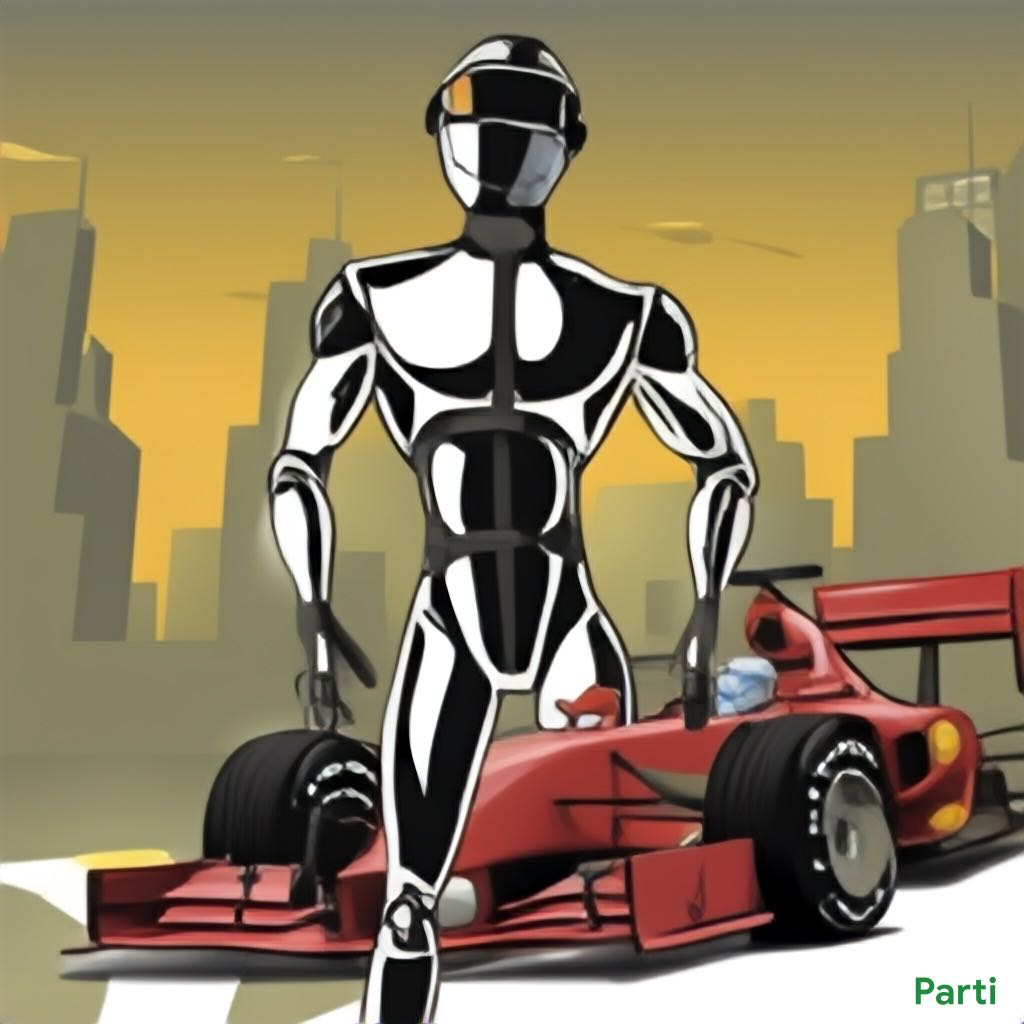
\includegraphics[width=\twobytwocolwidth\textwidth]{figures/limitations/robot_impossible.jpg}} &
\multicolumn{3}{c}{
\includegraphics[width=\twobytwocolwidth\textwidth]{figures/limitations/alien_impossible.jpg}} \\
\multicolumn{6}{C{\thirdcolwidth\textwidth}}{\tiny \textbf{G}. (a,b) Two images in the same batch for \textit{A horse sitting on an astronaut's shoulders. DSLR photo.} (c,d) Two images in the same batch for \textit{Zoomed out view of a giraffe and a zebra in the middle of a field covered with colorful flowers} \textbf{Failures}: hallucination (a); difficulty overriding strong priors (b); entity overriding (another horse instead of an astronaut) (b); entity duplication (zebras) (c,d).} && 
\multicolumn{6}{C{\thirdcolwidth\textwidth}}{\tiny \textbf{H}. (a,b) Two images generated in the same batch for \textit{A robot painted as graffiti on a brick wall. The words "Fly an airplane" are written on the wall. A sidewalk is in front of the wall, and grass is growing out of cracks in the concrete.} (c,d) Two images for \textit{a poodle wearing a baseball cap holding a dictionary in hand and writing bonez on a chalkboard} \textbf{Failures}: Errors/omissions in rendering text (all); use-mention confusion for words (b); incorrect visual aspect (grass)(a); displaced positioning (cracks) (a); hallucination (d).} && 
\multicolumn{6}{C{\thirdcolwidth\textwidth}}{\tiny \textbf{I}. (\textit{See main text for full prompts}) (a,b) Two images generated for a complex prompt of horses pulling a carriage, the statue of liberty, the moon, and the Earth, and images for (c) a robot race car driver and (d) alien graffiti with writing. \textbf{Failures}: Duplication of objects (a,b); relative scaling errors (a,b,c); physically impossible configurations (b,c,d); (unspecified) media blending (d).} \\


\end{tabular}
\end{adjustwidth}
\caption{Images from 20B \bdraw model showing errors and limitations. In the captions, (a), (b), (c), (d) refer to top left, top right, bottom left and bottom right, respectively. Note that many of the example images come from batches that included successful (and typically more highly ranked) images. See Section \ref{secs:limitations} for detailed discussion.}
\label{figs:limitations}
\end{figure}


\textbf{Color bleeding.} When color is provided for one object in a description or is very strongly associated with the object itself, but \textit{left unspecified for others}, it often spreads to the under-specified objects. Examples include baseballs being made yellow when in the presence of tennis balls (A(b,c)), or a crown being given the color of a shirt (D(a,d)).

\textbf{Feature blending.} Similarly, when two described objects have some similarities, they can become fused as one object or the attributes of another are incorporated. Examples included baseballs with tennis ball fuzz (A(b,c)), hybrids of the Great Pyramid and Mount Everest instead of co-placement (B(c,d)), and the melding of the VW symbol into the kilt's sporran (Fig. \ref{figs:cherry_tree}, boxes 4b, 4c, 5a).

\textbf{Omission, hallucination, or duplication of details.} Especially in complex scenes, the model will at times either omit some mentioned details, duplicate them or hallucinate things that are not mentioned. Examples include missing baseballs in A(d), the missing space shuttle in D(a,c), the missing horse carriage and statue in I(b), and the inclusion (hallucination) of glasses in H(d).

\textbf{Displaced positioning or interactions.} Objects are at times put in the wrong position (especially with increased prompt complexity). Examples include the beetle not grappling with the airplane in C(a,c,d), the space shuttle and drawing of a shuttle in D(b,d), the grass and crack in H(a), and the position of the Earth in I(b).

\textbf{Counting.} \bdraw can reliably produce up to seven objects of the same type (when not also specifying other objects as in panel A or mixing other details). Beyond that, it is mostly imprecise. When there are counts of multiple types of entities, there is a near complete failure, as shown in A(a-d). Interestingly, the reranker appears to help with counting; \eg for \textit{five red apples} the top six images all have five apples, but thereafter the count varies from four to six. For \textit{ten red apples} (see E(c,d)), the counts for the top-ranked eight images for one batch were \textit{8, 10, 9, 9, 9, 8, 11, 6}.

\textbf{Spatial relations.} While the model often correctly depicts objects specified as above or below each other, it is still inconsistent for that and is usually random for \textit{left} \vs\  \textit{right}. These failures especially compound when it involves spatial relations between groups of objects (e.g., A(a) and F(a,b)).

\textbf{Negation and absence.} \bdraw tends to draw items that are mentioned, even when the prompt says a thing is missing. For example, F(c,d) shows outputs that include bananas and orange juice even though the prompt is \textit{A plate that has no bananas on it. There is a glass without orange juice next to it.} F(d) has bananas off the plate, but this is just an incidentally interesting example and not an indicator of handling mention-of-absence well. We do find some examples with no bananas that are ranked very low, so there is also appears to be a compounding effect of both the generator and reranker in this case.

\textbf{Incorrect visual aspect and media blending.} Especially in scenes where mixed media types are involved, such as photo-realistic objects along with writing and paintings on walls, some items will jump from being depicted as an object to being depicted as a drawing, or vice versa. Examples include the drawn form of Anubis in D(a), the space shuttle as an object in D(b), and the grass as painted on the wall in H(a). We also see media blending, where an object's coherence is lost and it transitions from object to drawing, such as the blending of the drawn Anubis head with body in D(c) and the alien's top part being a painting that connects to non-drawn legs in I(d). While these are interesting visual effects, they were not specified in the prompt and thus indicate a lack of control over object coherence and appearance in such situations.

\textbf{Strong visual priors.} Certain configurations and visual features are so strongly correlated that it can be hard to nudge the model away from them, especially in the face of other complexities in the description. For example, Panel C shows a failed attempt to create a tank-sized rhinoceros beetle---for the most part, the model shrinks the scene (e.g. with a toy plane) or tries to use perspective to make the beetle appear visually larger. Its only successful attempt to make a massive beetle errs in including an actual tank. We also found that the model is very resistant to reverse a horse-and-rider situation: the only way to have the horse on the astronaut was to avoid \textit{riding} and instead rephrase this as something akin to \textit{a horse sitting on an astronaut's shoulders}; this produces some examples that give the requested configuration (G(a)), but most outputs contain errors, including the astronaut on the horse, the astronaut next to the horse, or even depicting the rider as a horse astronaut (G(b)). In some cases where a horse was put onto an astronaut, the model included yet another astronaut on the horse. As another example, when generating images of statues of Abraham Lincoln wearing clothing such as a polo shirt and a baseball cap, the model can do it reliably, but many of the outputs nevertheless have him wearing outfits from well-known statues and paintings of Lincoln.

\textbf{Strong linguistic priors.} Certain terms are highly associated with particular entities or word senses. For example, \textit{a soccer ball flying over a Lincoln} shows a ball flying over a statue of Abraham Lincoln. The automotive Lincoln can be brought in by adding \textit{car}, \textit{SUV}, etc. Similarly, \textit{a soccer ball flying over a bat} produces images of baseball bats; again, this can be fixed, as it were, by adding attributes of animal bats. It is even possible to explore the tensions between competing word senses in examples such as \textit{the astronomer married a star}, where the presence of astronomer invokes the heavenly body sense of \textit{star} but the act of marrying invokes (more plausibly) the sense of a movie star \cite{erk-herbelot-2021-marry}. When given \textit{an illustration of an astronomer marrying a star}, \bdraw goes with the heavenly body depiction, even when making it \textit{movie star}. Switching to a politician instead of astronomer leads to outputs showing a man and woman, but also including a star (iconic five-point representation) in the image. Even with more details such as \textit{A photo of an astronomer in a tuxedo marrying a beautiful movie star. The star is wearing a white dress.}, the model produces some outputs with a wedding couple, but backed by an image of the cosmos. It seems likely that the overwhelming presence of stars as heavenly bodies or icons in the visual training data creates a very strong combined linguistic and visual prior that is hard for the model to shift from. 

\textbf{Text rendering errors.} It is remarkable that text-to-image models like \bdraw and Imagen can render text in diverse and contextually appropriate ways on images (see the examples in Figure \ref{figs:cherries}, Panel F, for example), even though there is no explicitly curated or created training data for learning this ability. Nevertheless, text rendering is often hit-or-miss. It is common to have a few characters off even in simple prompts. For more complex prompts, the errors in rendering text increase with scene and descriptive complexity, as shown in Panel H. The ability to render text can also lead to situations where the model basically tries to render the entire prompt text in the image, e.g. as the title of a book. This usually happens for prompts that are not visually descriptive (e.g. \textit{How to succeed in life.}), and it is necessary to explicitly call out formats like \textit{oil painting} or \textit{illustration} in order for these to produce a non-textual output.

\textbf{Use-mention errors.} The model can render text on images, but at times it produces an image (use) rather than text (mention) (e.g., the drawing of an airplane in H(b)), or vice versa (rendering \textit{Space shuttle} on a t-shirt instead of drawing one -- another output related to D, but not shown).

\textbf{Disentangling multiple entities.} The model is often able to pack quite a lot of detail into an image that contains a single entity, but is much more challenged when there are multiple key entities. This can be seen with the sloth and van example of  Figure \ref{figs:cherry_tree}, where the model struggles at their combination (row 3, box b), and where subsequent addition of complexity leads to fewer good outputs. However, it is often even more difficult when the entities are of the same type, such as two animals, as demonstrated in E(a,b), where even fairly simple details are spread between the entities.

\textbf{Stylistic misses.} \bdraw can produce many styles reliably, such as pointillism and woodcut, but others like cubism and surrealism often miss the style at a deeper level, especially when applied to a complex scene. The styles of some specific painters can be modeled well, such as van Gogh and Rembrandt, but others are either lacking or very hit-or-miss, such as Michelangelo (which mostly look the same as adding \textit{oil painting}.). Interestingly, scale interacts with specific painters: for example, applying \textit{in the style of van Gogh} actually produces more diverse outputs consistent of style for the 3B model, while outputs are pretty much dominated by Starry Night with the 20B one.

\textbf{Impossible scenes.} Some outputs (usually ones ranked quite low) show entities that are inconsistently integrated, such as I(c), where the robot straddles the car in a nonsensical manner. Other cases involving mixed media lead to similarly bizarre outputs, including a drawing of Anubis's head on a photo-like body (D(c))  and a graffiti alien that extends to a depiction of real feet on the ground (I(d)). (Note that in both of these cases, these would be great outputs \textit{if} the prompt explicitly specified that these effects were desired.) Other challenges come up in trying to compose complex fantastical scenes, such as the carriage, moon and earth outputs in I(a,b), where the lighting of the statue, moon and Earth are completely inconsistent (a) and the Earth appears sitting on the moon (b).

\textbf{Zoom and perspective.} \bdraw often produces outputs that are too zoomed in, e.g. showing just part of a vehicle or a subject. While it can respond to directives like \textit{zoomed out}, \textit{three-quarters view}, \textit{wide-angle lens}, this still often results in cropping on the subject. To ensure broader view, it is often necessary instead to use other details, such as including shoes on a subject to get the feet or adding a description of a field and flowers to get an entire giraffe (as done in G(c,d)).
     
\textbf{Animal protagonists.} Due to concerns discussed in Section~\ref{secs:broader}, we experimented with many animals acting as stand-ins for protagonists in descriptions. As it turns out, some animals are easier to work with than others. For example, mammals with paws that are more similar to human hands, such as bears, wombats, and raccoons more reliably result in better images than geckos, insects, and fish. This is likely due to the visual and morphological similarity they have with people as well as the fact that they are more commonly used as human-like protagonists in the wider visual world (\eg, in cartoons). It is also often necessary to include ``photo'' or ``photograph'' in the prompt to push the model to make photo-like images, and even then it will often produce cartoon-like outputs---especially with increasing description complexity.

\textbf{Detailed or tricky visual effects.} It is very difficult to get the model to respond to prompts such as \textit{a bear emerging from a puzzle} (and variations thereof) where one might want to have an Escher-like image of part of the bear appearing as quasi-real and the other being part of the puzzle. In general, controlling such fine-grained specifications seems beyond the current model, and is likely to be better served in an interactive editing setting.
    
\textbf{Common misconceptions.} Some visual world knowledge is incorrectly understood in the broader world, and this is partially reflected in the data and then the model. For example, it is commonly thought that the central pyramid in the Giza Complex is the Great Pyramid, but in fact that is the pyramid of Khafre. The true Great Pyramid is Khufu's, which is to the north. Khafre's pyramid is often mistakenly attributed as the \textit{great one} because it sits on slightly higher ground (but is actually shorter at 136.4 meters compared to Khufu's 146.6 meters) and because it sits prominently behind the Great Sphinx. This mistaken attribution is reflected in images associated with the terms \textit{the Great Pyramid}, and it shows up in many of \bdraw's outputs for the Great Pyramid (including B(d)).

We hope these observations and breakdown of limitations and error types, and their correspondences in many of the \bcp, will be useful both for contextualizing the strong capabilities we present elsewhere in the paper and for inspiring future work on improving text-to-image generation models in general. In this light, it is also worth recalling WordsEye \cite{coyne2001wordseye}, an automatic text-to-scene system built in 2001. It derived dependency structures from prompts, converted them to semantic structures, and then used those to select, position and scale the objects and participants in the described scene. Though it is no match for current text-to-image such as \bdraw on open-domain, broad capabilities, including world knowledge, it actually could \textit{precisely} manage several of the above stated limitations, including counting, negation, relative scale, and positioning -- such that it could produce a computer graphics visual (based on an explicit 3D representation) corresponding to complex prompts such as:

\begin{quote}
John uses the crossbow. He rides the horse by the store.The store is under the large willow. The small allosaurus is in front of the horse. The dinosaur faces John. A gigantic teacup is in front of the store. The dinosaur is in front of the horse. The gigantic mushroom is in the teacup. The castle is to the right of the store.
\end{quote}

\noindent
WordsEye could also handle specifications of measurements such as lengths and heights, and make correct visual adjustments for the output image, \eg, for prompts such as \textit{The lawn mower is 5 feet tall. John pushes the lawn mower. The cat is 5 feet behind John. The cat is 10 feet tall.} With the advent of broadly capable -- but often imprecise models -- such as Dall-E 2, Imagen and \bdraw, this should inspire us to revisit ideas and capabilities of earlier systems such as WordsEye and aspire toward models that combine breadth, visual quality, and control.
